% REMEMBER: You must not plagiarise anything in your report. Be extremely careful.

\documentclass{l4proj}

    
%
% put any additional packages here
%
\usepackage{booktabs}
\usepackage{pdfpages}
\usepackage{float}
\begin{document}

%==============================================================================
%% METADATA
\title{Improved Steganography Algorithm}
\author{Daniel Hislop}
\date{25th January 2021}

\maketitle

%==============================================================================
%% ABSTRACT
\begin{abstract}
    Steganography is the practice of concealing information to perform secret communication. As time has progressed, steganography has evolved from the physical to the digital domain. Simple techniques such as Least Significant Bit (LSB) steganography perform such concealment with a relatively small amount of data. The Bit-Plane Complexity Segmentation (BPCS) algorithm takes advantage of properties of human vision to increase the embeddable amount. 

    BPCS possesses vulnerabilities that leave it vulnerable to digital detection. This paper identified a vulnerability in the histogram of block complexities, where the conjugation process produces blocks of high complexity not present in natural images. Two modifications address the problems arising from BPCS embedding. These are variable complexity and random bitplane embedding order. For the former, complexity thresholds vary between bitplanes during embedding, rather than a single static measure used in the standard BPCS algorithm. For the latter, random bitplane embedding order (RBEO) changes the order of bitplanes in which we conceal data. In the standard BPCS algorithm, we embed from the least significant bitplane to the most significant bitplane. RBEO randomises this order. 
    
    Analysis of the impact of these modifications occurred in two stages. First, a visual detection phase in which external participants gave a verdict on whether they believed a hidden payload was present in the image displayed to them. These comprised six clean images, six stego objects created through the standard BPCS algorithm, six through variable complexity and six through RBEO. An equal performance between the standard algorithm and variable complexity came in the form of 43.33\% correct guesses. RBEO saw the worst performance, with 96.67\% of images guessed correctly. Secondly, using a novel digital detection tool, these images were supplied as parameters resulting in a verdict of "Hidden payload" or "No Hidden payload". A reduction in the 100\% detection rate for the standard algorithm to 66\% for variable complexity marks a $\sim$33\% improvement. RBEO again made no positive impact.
    
    Additionally, the paper investigates the effects of lossy compression using the JPEG algorithm on steganography. We hide data using three techniques, Least Significant Bit, Third Least Significant bit and Third Least Significant bit Random. Due to the low embedding capacity of 12.5\%, most images in the test bank were unsuitable for the task. Thus, LSB techniques following JPEG compression are less appropriate for secret communication than that of BPCS. Finally, an evaluation of the compression process itself took place. Such an evaluation considered two metrics relating to the compressed image: mean square error and peak signal to noise ratio. Metric values were in line with those found in external literature. Meaning the compression performed produces images of sufficient quality, comparable to those seen elsewhere.
\end{abstract}

%==============================================================================

% EDUCATION REUSE CONSENT FORM
% If you consent to your project being shown to future students for educational purposes
% then insert your name and the date below to  sign the education use form that appears in the front of the document. 
% You must explicitly give consent if you wish to do so.
% If you sign, your project may be included in the Hall of Fame if it scores particularly highly.
%
% Please note that you are under no obligation to sign 
% this declaration, but doing so would help future students.
%
\def\consentname {Daniel Hislop} % your full name
\def\consentdate {25th January 2021} % the date you agree
%
\educationalconsent
%==============================================================================
\newpage
\chapter*{Acknowledgements}

I would like to express my gratitude toward my supervisor Dr Ron Poet for his continuous support, advice and assistance throughout the project.  
\clearpage



%==============================================================================
\tableofcontents

%==============================================================================
%% Notes on formatting
%==============================================================================
% The first page, abstract and table of contents are numbered using Roman numerals and are not
% included in the page count. 
%
% From now on pages are numbered
% using Arabic numerals. Therefore, immediately after the first call to \chapter we need the call
% \pagenumbering{arabic} and this should be called once only in the document. 
%
% Do not alter the bibliography style.
%
% The first Chapter should then be on page 1. You are allowed 40 pages for a 40 credit project and 30 pages for a 
% 20 credit report. This includes everything numbered in Arabic numerals (excluding front matter) up
% to but excluding the appendices and bibliography.
%
% You must not alter text size (it is currently 10pt) or alter margins or spacing.
%
%
%==================================================================================================================================
%
% IMPORTANT
% The chapter headings here are **suggestions**. You don't have to follow this model if
% it doesn't fit your project. Every project should have an introduction and conclusion,
% however. 
%
%==================================================================================================================================
\chapter{Introduction} \label{Introduction}

% reset page numbering. Don't remove this!
\pagenumbering{arabic} 

\section{Motivation}


Throughout history, humans have devised various methods of concealing information to perform secret communication. This practice is known as steganography. Steganography differs from practices like cryptography that opt to encipher data by instead masking its presence. The earliest example dates back to 499BC; Histiaeus, a Greek ruler, orchestrated a revolt by way of tattooing the head of a slave, waiting for his hair to grow back and sending him to the receiver who would then shave the head; to reveal the hidden message \citep{histiaeus}. With rapid technological advancement, steganography has followed suit, expanding from the physical to the digital domain. Audio, text, video and image files all serve as suitable carriers for secret information.

Simple techniques such as Least Significant Bit (LSB) steganography offer a method of concealing information, albeit with a relatively small amount of data. \citet{Kawaguchi1999PrinciplesAA} proposed the Bit-Plane Complexity Segmentation (BPCS) algorithm, having a distinct advantage over LSB steganography through a significantly increased hiding capacity. However, BPCS is not without its flaws; information concealed using BPCS remains susceptible to digital detection. An important point to consider is that the JPEG image format is the most likely to appear in the wild. Information embedded will not persist due to the lossy compression employed by the JPEG algorithm. As a result, the embedding process requires different steganographic techniques to account for this. 

 
\section{Aims}

\begin{itemize}
    \item \textbf{Identify Vulnerabilities}: Aspects of the algorithm produce identifiable signatures, increasing the likelihood of detection when performing digital analysis. The project will identify these and discuss the reasons for their effect.
    \item \textbf{Rectify Vulnerabilities}:  Addressal of the previously identified vulnerabilities through the addition of modifications to the BPCS algorithm.
    \item \textbf{Create Detection Tool}: The development of an automated tool capable of detecting hidden payloads within images using a range of steganalysis techniques. 
    \item \textbf{Evaluate Improvements}: Assess the impact of the modifications on the perceptibility of hidden payloads. A series of metrics such as the detection rate of the previously discussed tool allows for this. 
    \item \textbf{JPEG Compression}: The project will implement JPEG compression to facilitate an investigation into subsequent steganographic techniques.
    \item \textbf{JPEG Steganography}: The project will investigate how the JPEG algorithm affects the steganographic techniques required to conceal information and then implement them. 
\end{itemize}
%==================================================================================================================================
\chapter{Background} \label{Background}

\section{Literature Review}

\citet{Schyndel1994ADW} proposed a mechanism for digital watermarking of images, involving a substitution in the least significant image bitplane. A watermark serves as image identification as an original or legitimate source. Through experimentation on 8-bit colour images, the authors found LSB to be a reliable and straightforward way of achieving said goals. As development in the field progressed, it was readily apparent that statistical analysis could easily defeat LSB steganography.  \citet{1337281} performed hypothesis testing in combination with a probability mass function to determine the presence of concealed information. Despite consistent detection, performance decreased for images with relatively low amounts of embedded data. Additionally, more recent contributions by \cite{https://doi.org/10.1002/sec.864} involved a theoretical approach to identifying LSB embedding characteristics in the image histogram of multi-order differences. It found LSB to smooth such a graph.

Parallel to LSB's introduction, \citet{Kawaguchi1999PrinciplesAA} outlined the BPCS algorithm and investigated the technique experimentally to evaluate its effectiveness. The key novelty of the algorithm was exploiting properties of the human visual system to embed data. This paper expanded on existing work in the field. The concept of "complexity" was derived from \citet{0e8da7e9d1d74bc291f3f5edeb11d513}, further reinforced by the work of \citet{kawaguchi1997modeling}. BPCS's innovation led to wider usage, incentivising work in steganalysis. \citet{shuozhong2005statistical} noted clear signs of BPCS embedding in the complexity histograms of images. Due to this, the modification of different complexity thresholds per bitplane was presented in \citet{sun_2015}.

As a result of the vulnerabilities in the algorithm, there has been a move to create improvements. Either they were attempting to increase payload capacity or decrease digital detection. Much like an adaptive complexity threshold, this idea applies to the block size itself. \citet{Patel2014ImageSS} implemented an adaptive BPCS algorithm that would split an image into 4x4, 8x8, and 16x16 blocks. That allowed for a higher embedding capacity. 

Lossy compression used in the JPEG algorithm means different considerations for the techniques used. However, we can still retain a simple steganography form like LSB and adapt it to the situation. \citet{Morsy} performed embedding in the least significant bit of the DCT coefficients of JPEG images. The adapted technique "maximizes the ratio between even and odd DCT coefficients so as to preserve the first order statistics of JPEG images"\citep{Morsy}. One work of interest is a technique to resist the JPEG algorithm's compression to ensure the embedded message survives the process. \citet{doi:10.1080/02564602.2018.1476192} explored this robust method. This motivation differs from others that would embed the data after compression; however, this purports to survive the compression process.

LSB steganography's main issue is the meagre capacity; while LSB may be appropriate for watermarking, it is not quite so for secret communication. \citet{westfeld2001f5}  presented the F5 steganography algorithm to address the issue, claiming to not increase the likelihood of successful visual and digital attacks. Further exploration of the F5 algorithm led to reliable detection using a multi-class classifier that uses "combined DCT and Markov features" presented by \citet{10.1117/12.696774}. F5 is an included algorithm in this. However, it is also capable of detecting well-regarded algorithms like Steghide and JP Hide&seek.

\section{Fundamental Concepts}

\subsection{Pixels}

When we look at images, it is easy to draw clear distinctions. Consider figures \textbf{\ref{fig:dog_image}} and \textbf{\ref{fig:cat_image}}, there is a readily apparent difference between the meaning conveyed, colours and objects themselves. Despite this, these two images are represented in the same fashion by the computer.

\begin{figure}[!h]
    \centering
    \begin{subfigure}[b]{0.4\textwidth}
        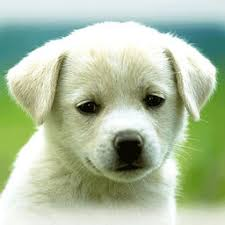
\includegraphics[width=\textwidth]{images/dog.jpg}
        \caption{A 256x256 image of a dog}
        \label{fig:dog_image}
    \end{subfigure}
    \begin{subfigure}[b]{0.4\textwidth}
        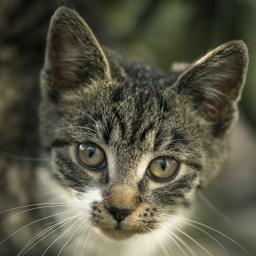
\includegraphics[width=\textwidth]{images/cat.jpg}
        \caption{A 256x256 image of a cat}
        \label{fig:cat_image}
    \end{subfigure}
    \caption{Two 256x256 Images. \subref{fig:dog_image} shows an image of a dog. \subref{fig:cat_image} shows an image of of a cat.}
\end{figure}

Each is composed of an array of fundamental units known as pixels of different numerical values. In an 8-bit colour image, typically referred to as a grayscale image, a pixel value will range between 0 and 255, where 0 indicates white and 255 indicates black - with those in-between representing varying shades of grey. Figure \textbf{\ref{fig:hex_chart}} shows a hexadecimal chart of the colour of each pixel value. RGB images differ in that they are composed of three channels, red, blue and green. Each channel has a numerical value that is combined to produce a single pixel value. 

\begin{figure}[!h]
    \centering
    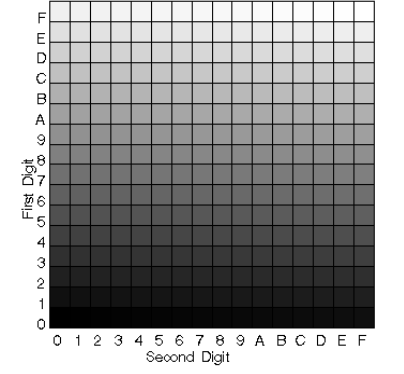
\includegraphics[width=10cm, height=10cm]{images/pixel_hex_chart.png}
    \caption{A chart of of pixel colours with their respective Hexadecimal representation. Sourced from \citet{singh2015steganography}}
    \label{fig:hex_chart}
\end{figure}


\subsection{What are bitplanes?}

Numerical values are expressible in a binary representation. Consider the following example:

Taking the pixel value of 32 translates in 8-bit binary as 00100000. Each bit in this 8-bit representation is known as a bitplane, as shown as follows:

\begin{table}[!h]
\begin{tabular}{|l|l|l|l|l|l|l|l|l|}
\hline
Bit & 0 & 0 & 1 & 0 & 0 & 0 & 0 & 0 \\ \hline
Bitplane & 1st & 2nd & 3rd & 4th & 5th & 6th & 7th & 8th \\ \hline
\end{tabular}
\end{table}

\subsection{Terminology}
\begin{itemize}
    \item Cover - The image used to conceal our secret communication.
    \item Payload - The data to be embedded.
    \item Stego -  The object produced by embedding the payload within the cover object.
\end{itemize}

\section{LSB Steganography}

LSB Embedding \citep{Morsy} is a simple form of steganography performed by replacing the rightmost bit, known as the least significant bit, of cover object pixels with a payload bit. Substitution of this LSB will lead to a change in the pixel value of at maximum, 1. Such a small change is beneficial as it ensures changes to the cover image are not susceptible to visual detection. Illustrating with an example:

A pixel value of 198:
\begin{table}[!h]
\begin{tabular}{|l|l|l|l|l|l|l|l|}
\hline
1 & 1 & 0 & 0 & 0 & 1 & 1 & 0 \\ \hline
\end{tabular}
\end{table}

We embed 1 in the least significant bit. Giving us a pixel value of 199:

\begin{table}[!h]
\begin{tabular}{|l|l|l|l|l|l|l|l|}
\hline
1 & 1 & 0 & 0 & 0 & 1 & 1 & 1 \\ \hline
\end{tabular}
\end{table}

\begin{figure}[!h]
    \centering
    \begin{subfigure}[b]{0.45\textwidth}
        
\includegraphics[width=\textwidth]{images/pixel_val_198.png}
        \caption{Pixel value 198 colour}
        \label{fig:pixel_value_198}
    \end{subfigure}
    \begin{subfigure}[b]{0.45\textwidth}
        
\includegraphics[width=\textwidth]{images/pixel_val_199.png}
        \caption{Pixel value 199 colour}
        \label{fig:pixel_value_199}
    \end{subfigure}
    \caption{Effect of LSB substitution on pixel value. Figure \subref{fig:pixel_value_198} shows the colour of pixel value 198. Figure \subref{fig:pixel_value_199} shows the colour of pixel value 199.}
\end{figure}

As a result of this operation, we have been able to embed data in the least significant bit, leading to a pixel value change that is visually undetectable. Figure \textbf{\ref{fig:pixel_value_198}} shows the colour of the unchanged cover pixel, and figure \textbf{\ref{fig:pixel_value_199}} is the resultant colour after embedding. The two shades are the same to the human eye. 

\section{BPCS Steganography}

Images are composed of "informative" and "noise-like" regions. The categorisation of an image region into one of its two possible types is dependent on its complexity value. Region complexity is a measure of the frequency of colour changes. We perform a calculation to derive this value by dividing the colour changes row-wise and column-wise by the maximum possible number of colour changes. A checkerboard pattern of 1s and 0s exhibits this maximum number.

What exactly do these categorisation terms mean? A noise-like region is one in which we can safely alter a significant portion of data without distorting the given area. Conversely, the substitution of data from parts of the image deemed informative is more likely to introduce noticeable visual degradation. First, we set a complexity threshold, typically of value 0.3. 
Region complexity measures greater than this chosen value fit the "noise-like" definition, whereas those less than fall into the "informative" category. Respectively, we refer to such regions as complex and non-complex.

It is possible to convert a region's category to the alternative, i.e. noise-like to informative and vice-versa. This transformation is known as the conjugation operation. In this, we take the logical XOR of our region and a checkerboard pattern, resulting in a new complexity measure of 1 - x, where x is the original complexity value.

During BPCS embedding, we first convert our array of pixel values from their binary representation into gray coding. Gray coding \citep{what_is_gray_code?_2021} is an alternative ordering of the standard binary form of numbers. Such that a difference of 1 in numerical representation will reflect only one change in the bit representation. Following this, we split both the cover and payload objects into 8x8 blocks for each of the eight bit-planes. Complex regions in the cover get replaced with 8x8 payload blocks. Should any replacement of a cover block produce a new non-complex block, the block is conjugated. A record of conjugations, known as the conjugation map, is also embedded within the cover object. After successful embedding, we convert from gray coding back to standard binary representation. 

\section{JPEG Algorithm}\label{jpeg_overview}

In 1992, the Joint Photographic Experts Group developed the JPEG algorithm \citep{lossy_data_compression:_jpeg_2021}. Various standards of the algorithms exist. However, the baseline implementation is the concern of the project scope. The baseline is defined as follows: Convert to YCbCr colour space, split an image into 8x8 blocks, perform the Discrete Cosine Transform (DCT) on each block, normalise the resulting DCT coefficients with an appropriate quantization matrix,  perform zigzag encoding and finally run-length encoding.

\subsection{Discrete Cosine Transform}

The Discrete Cosine Transform \citep{the_discrete_cosine_transform_(dct)_2021} is a mathematical operation that acts on the image we have by transforming it from the spatial domain to the frequency domain. The spatial domain refers to the 2D matrix of pixel values, whereas the frequency domain refers to the rate of changes in pixel values. \citep{spatial}. Consider some arbitrary data and the cosine functions in figures \textbf{\ref{fig:cosx}} and \textbf{\ref{fig:cos2x}}. We can think of DCT as expressing an approximation of the data in terms of these differing cosine functions. In the actual JPEG DCT, 64 basis functions, displayed in figure \textbf{\ref{fig:dct_basis_functions}}, are used in place of the arbitrary cosine functions seen previously. Each function can be said to be of different "weighting", indicating the extent to which each contributes to reproducing the data. The DCT coefficients are the weighting factors of each of these basis functions. JPEG compression saves storage space by removing the cosine functions that make little contribution to the image.

\begin{figure}[]
    \centering
    \begin{subfigure}[b]{0.35\textwidth}
        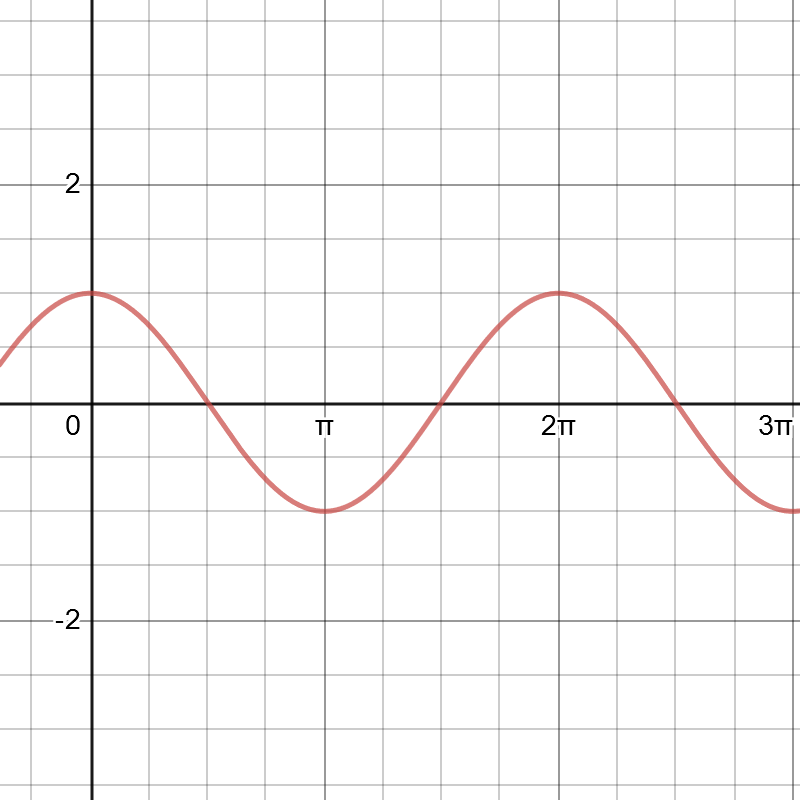
\includegraphics[width=\textwidth]{images/cosine_x_graph.png}
        \caption{Cosine function x}
        \label{fig:cosx}
    \end{subfigure}
    \begin{subfigure}[b]{0.35\textwidth}
        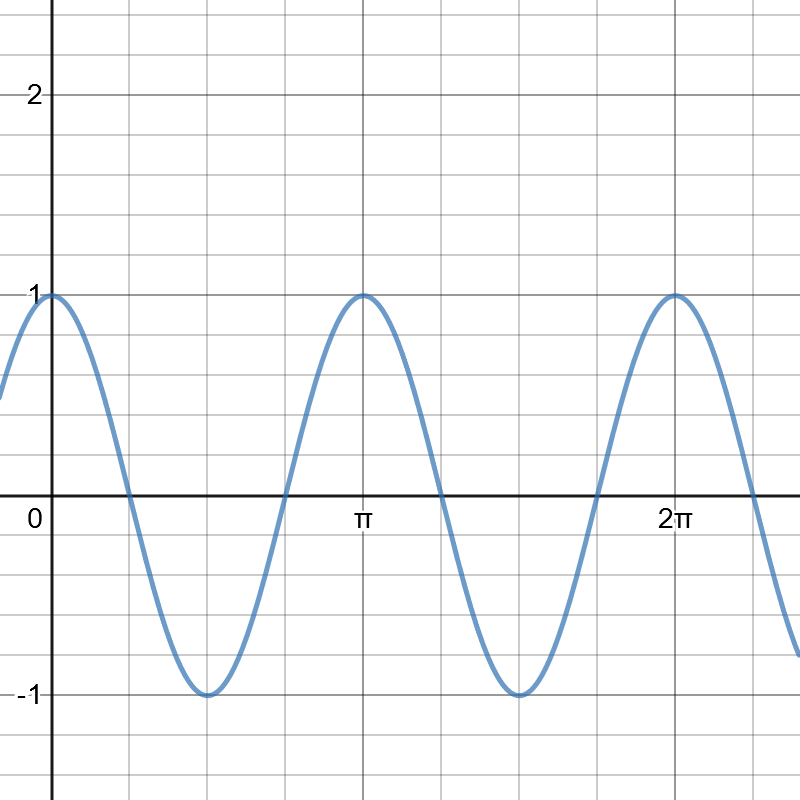
\includegraphics[width=\textwidth]{images/cosine_2x_graph.png}
        \caption{Cosine function 2x}
        \label{fig:cos2x}
    \end{subfigure}
    \begin{subfigure}[b]{0.35\textwidth}
        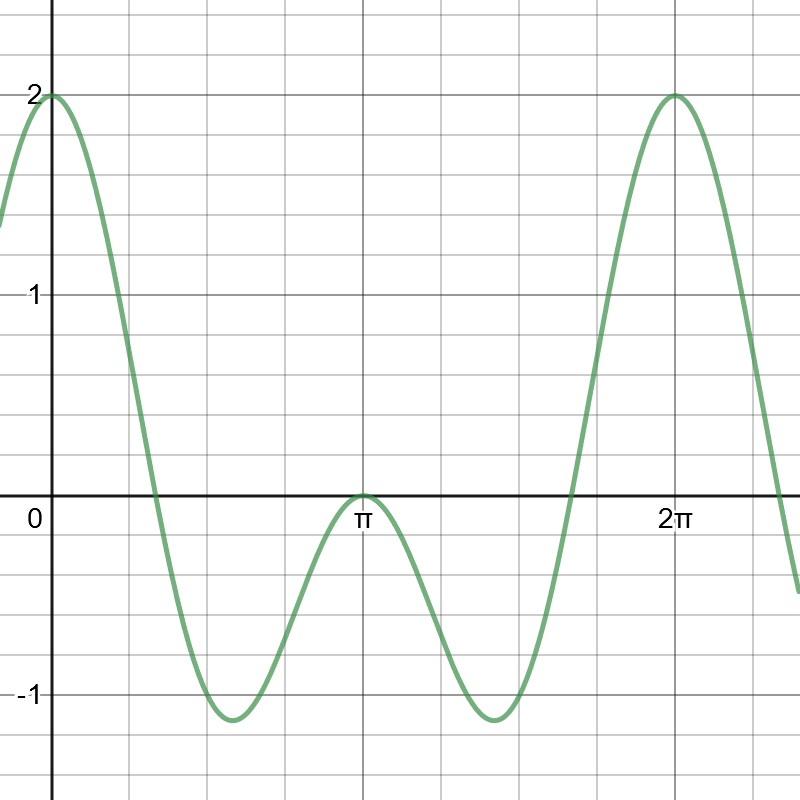
\includegraphics[width=\textwidth]{images/cosine_sum_graph.png}
        \caption{Cosine function Sum}
        \label{fig:cos_sum}
    \end{subfigure}
    \begin{subfigure}[b]{0.35\textwidth}
        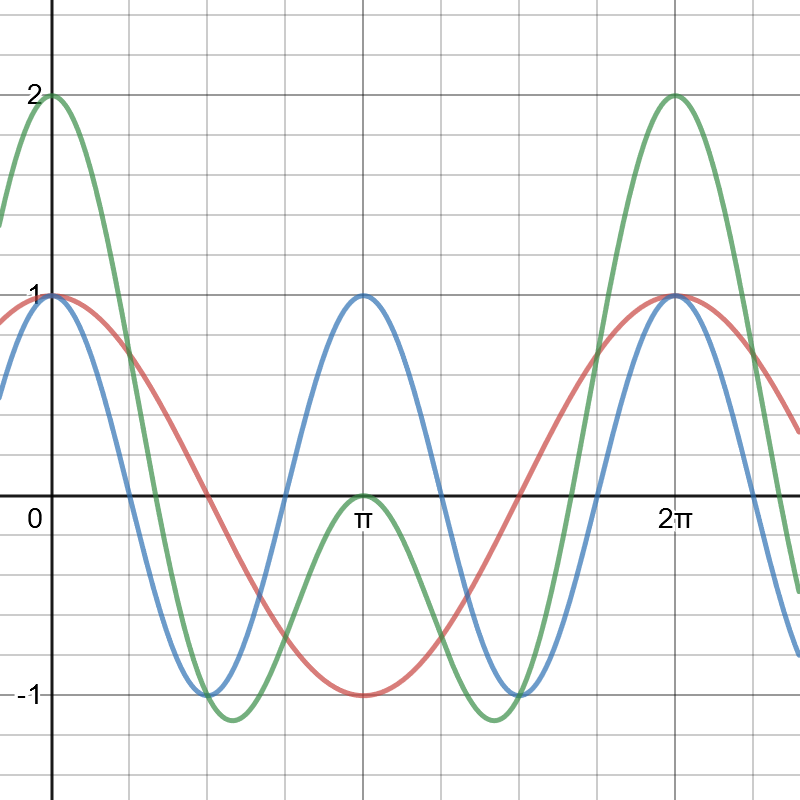
\includegraphics[width=\textwidth]{images/cosine_all_graph.png}
        \caption{Cosine function All}
        \label{fig:cos_all}
    \end{subfigure}
    \caption{Visualisations of cosine functions. Figure \subref{fig:cosx} shows cosine function x. Figure \subref{fig:cos2x} shows cosine function 2x, Figure \subref{fig:cos_sum} shows the sum of the two cosine functions. Figure \subref{fig:cos_all} shows all cosine functions. }
\end{figure}

\begin{figure}[]
    \centering
    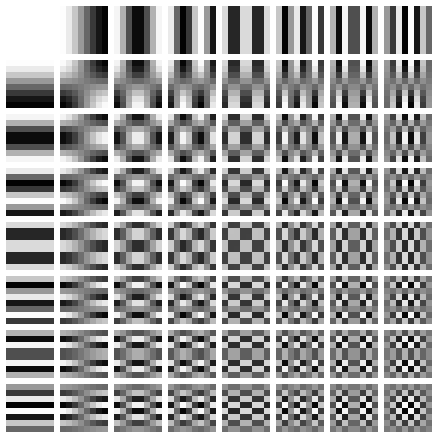
\includegraphics[width=0.3\textwidth]{images/dct_basis_functions.png}
    \caption{The 64 (8x8) Cosine basis functions in the Discrete Cosine Transform. Sourced from \citet{khalid_2021}.}
    \label{fig:dct_basis_functions}
\end{figure}

\subsection{DC vs AC Coefficients}

In our 8x8 block of DCT coefficients, we have one direct coefficient (DC), the first value in the matrix, and 63 alternating coefficients (AC). The DC coefficient represents the region's average colour value. The AC coefficients represent the colour changes across the block. Coefficients furthest away from the DC contribute less to producing the approximation of the original data. 

\subsection{Quantization}

JPEG achieves lossy compression through the use of the quantization process. Following the calculation of DCT coefficients, we normalise with a quantization table. Default tables exist for this purpose, although these will typically vary between organisations and applications such as Photoshop and image software provided by camera companies like Canon. To normalise, we divide the coefficients by either the chrominance or luminance quantization tables, where appropriate, shown in table \textbf{\ref{q_matrices}}. Typically, this leads to a reduction in the high-frequency components, the AC coefficients furthest from the DC coefficient, to zero, resulting in an approximation of the data with reduced storage requirements.

\begin{table}[!htb]
    \caption{Default Quantization Tables for Chrominance and Luminance components - Tables reconstructed from those presented by \citet{attaby_2021}}
    \begin{minipage}{.5\linewidth}
      \caption{Chrominance Quantization Matrix}
      \centering
        \begin{tabular}{|l|l|l|l|l|l|l|l|}
            \hline
            16 & 11 & 10 & 16 & 24  & 40  & 51  & 61  \\ \hline
            12 & 12 & 14 & 19 & 26  & 58  & 60  & 55  \\ \hline
            14 & 13 & 16 & 24 & 40  & 57  & 69  & 56  \\ \hline
            14 & 17 & 22 & 29 & 51  & 87  & 80  & 62  \\ \hline
            18 & 22 & 37 & 56 & 68  & 109 & 103 & 77  \\ \hline
            24 & 35 & 55 & 64 & 81  & 104 & 113 & 92  \\ \hline
            49 & 64 & 78 & 87 & 103 & 121 & 120 & 101 \\ \hline
            72 & 92 & 95 & 98 & 112 & 100 & 103 & 99  \\ \hline
        \end{tabular}
    \end{minipage}%
    \begin{minipage}{.5\linewidth}
      \centering
        \caption{Luminance Quantization Matrix}
        \begin{tabular}{|l|l|l|l|l|l|l|l|}
            \hline
            17 & 18 & 24 & 47 & 99 & 99 & 99 & 99 \\ \hline
            18 & 21 & 26 & 66 & 99 & 99 & 99 & 99 \\ \hline
            24 & 26 & 56 & 99 & 99 & 99 & 99 & 99 \\ \hline
            47 & 66 & 99 & 99 & 99 & 99 & 99 & 99 \\ \hline
            99 & 99 & 99 & 99 & 99 & 99 & 99 & 99 \\ \hline
            99 & 99 & 99 & 99 & 99 & 99 & 99 & 99 \\ \hline
            99 & 99 & 99 & 99 & 99 & 99 & 99 & 99 \\ \hline
            99 & 99 & 99 & 99 & 99 & 99 & 99 & 99 \\ \hline
            \end{tabular}
    \end{minipage} 
    \label{q_matrices}
\end{table}

\subsection{Zig-Zag Encoding}\label{zig-zag}

Zig-Zag encoding is a reordering of coefficients such that those of lowest frequency appear closer to the DC, while high-frequency coefficients, reduced to zero, will be grouped at the end. Zig-Zag encoding's main benefit is apparent in the subsequent step of the compression process, discussed in section \textbf{\ref{RLE}}. Figure \textbf{\ref{fig:zig_zag_pattern}} shows the zig-zag pattern performed during traversal of the normalised coefficients matrix.

\begin{figure}[]
    \centering
    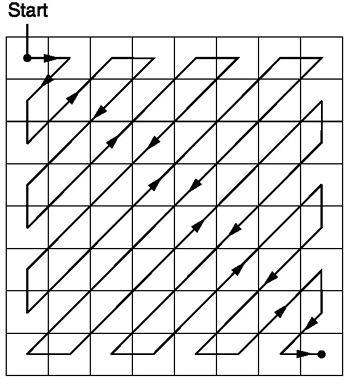
\includegraphics[width=0.4\textwidth]{images/zigzag_pattern.jpg}
    \caption{Zig-Zag pattern traversal of 8x8 block of DCT coefficients. Sourced from \citet{khalid_2021}.}
    \label{fig:zig_zag_pattern}
\end{figure}

\subsection{Run Length Encoding}\label{RLE}

Run Length Encoding is one mechanism for performing lossless compression, differing from the lossy compression in the quantization step. RLE functions by representing data in terms of consecutive occurrences of values. As an example, 0000000000 in RLE would be 0 10, i.e. a value of zero consecutively occurring ten times. When applied over a large dataset, RLE's use leads to a dramatic reduction in storage requirements. Its use is readily apparent after considering the zig-zag traversal discussed in section \textbf{\ref{zig-zag}} which groups high-frequency components, reduced to zero, together.

\section{Steganalysis}\label{steganalysis}

Steganalysis is the area of study encompassing the methods of hidden payload detection, both physical and digital. Some steganographic techniques create embedding signatures in the stego objects produced. Steganalysis seeks to exploit these vulnerabilities. In the steganalysis technique presented by \citet{valley}, statistical analysis involves the generation of a complexity histogram. This histogram is a probability distribution of the complexity measures of blocks in the image. Substitutions of payload blocks into a cover object will affect this distribution, whereby there will be a noticeable difference between the complexity histograms of natural images and BPCS embedded images. We can plot the histogram for each bitplane in the image; a tampered image will show a reduced probability of blocks having a complexity measure at the chosen complexity measure, or as a visual cue; a "valley-like" signature will appear around the threshold.

\section{Summary}

This chapter presented an overview of existing literature within the field. A review of this lent itself to a subsequent explanation of relevant fundamental concepts and algorithm steps. Information presented here serves as the required background knowledge to understand ensuing ideas.

%==================================================================================================================================
\chapter{Analysis/Requirements} \label{Analysis}

Through communication with the project supervisor and supplementary background reading, the project requirements comprise both functional and non-functional requirements. Subsequently, this led to a prioritisation using the MoSCoW method \citep{moscow}. Choosing this technique ensured that central ideas of concern would have higher proportions of time allocated.  

In MoSCoW, requirements are labelled as the following:
\begin{itemize}
    \item Must have - The project is deemed unsuccessful if any of these are not met.
    \item Should Have - Project success is not contingent upon the inclusion of these requirements. However, failure to implement them will mean losing out on a significant portion of utility.
    \item Could Have - Typically small additions that offer utility, however, the project can function if they are missed.
    \item Would like to have - Requirements that are relevant to the project specification but will only be implemented over the course of the current development life-cycle if time is available at the end.
\end{itemize}

\section{Functional Requirements}\label{functional_requirements}

Functional requirements are defined as requirements "that must be implemented to enable users to accomplish their tasks" \citep{functional_non_functional}. We label functional requirements using the acronyms: \textbf{MH}, \textbf{SH}, \textbf{CH} and \textbf{WH} to reflect Must Have, Should Have, Could Have, and Would like to have, from the MoSCoW prioritisation method.

\begin{enumerate}
    \item \textbf{MH} - Standard BPCS Algorithm. Implementation in a programming language of choice of the standard algorithm defined by \citet{Kawaguchi1999PrinciplesAA}.
    \item \textbf{MH} - One modification to the BPCS algorithm. There must be a modification to the BPCS algorithm that attempts to improve resistance to digital detection.
    \item \textbf{MH} - Detection Tool - A detection tool developed in a language of choice must exist to facilitate the evaluation of the BPCS modification against the standard algorithm. The metric from its usage will be the detection rate. 
    \item \textbf{MH} - JPEG compression algorithm - Implementation of the baseline standard JPEG algorithm. We define the standard as splitting an image into 8x8 blocks, performing DCT, quantization, zigzag encoding and run-length encoding.    
    \item \textbf{MH} - Implementation of one JPEG steganographic technique in either the spatial or frequency domain. 
    \item \textbf{MH} - BPCS Tool functionality for 8-bit colour images.
    \item \textbf{MH} - JPEG compression functionality for 8-bit colour images.
    \item \textbf{MH} - JPEG steganography functionality for 8-bit colour images.
    \item \textbf{MH} - Detection Tool functionality for 8-bit colour images.
    \item \textbf{SH} - Second modification to the BPCS algorithm - Two modifications were asked of by supervisor at the outset of the project. Only one is required for an evaluation to take place, however two should be implemented. 
    \item \textbf{SH} - Further evaluation metrics - Metrics pertaining to the quality of images compressed by the JPEG tool should be reported on.
    \item \textbf{SH} - BPCS Tool functionality for 24-bit colour images.
    \item \textbf{SH} - JPEG compression functionality for 24-bit colour images.
    \item \textbf{SH} - JPEG steganography functionality for 24-bit colour images.
    \item \textbf{SH} - Detection Tool functionality for 24-bit colour images.
    \item \textbf{CH} - Steps beyond the JPEG baseline standard such as Huffman Encoding could be implemented in the JPEG tool. 
    \item \textbf{CH} - Second JPEG steganographic technique - The domain not chosen to meet the "SH" requirement for JPEG steganography could be implemented. As an example, if the spatial domain was chosen for "SH", then steganography in the frequency domain would meet the "CH" requirement.

\section{Non-Functional Requirements}\label{non_functional_requirements}

Non-Functional requirements are defined as requirements that "describe how a system must behave and establish constraints of its functionality" \citep{functional_non_functional}. Like before, these will be labelled using the acronyms: \textbf{MH}, \textbf{SH}, \textbf{CH} and \textbf{WH}. 

    \item \textbf{MH} - Documentation - Extensive documentation of the system for users and future developers. Enables system usage and allows for a future developer to understand each component of the system.
    \item \textbf{SH} - Modularity - The developed system must be modular to allow future work directly on an individual component without reliance on the other tools in the system. As an example, future work focuses on adding further modifications to the algorithm in the BPCS tool. 
    \item \textbf{SH} - Extensibility - The developed system should facilitate future work without requiring significant changes to the underlying architecture. 
    \item \textbf{SH} - Testing - Creation of unit test cases to signal where and why errors occur during system usage. 
    \item \textbf{CH} - Portability - The system should be able to be used on both Linux and Windows operating systems.
\end{enumerate}

\section{Summary}

This chapter detailed the requirements analysis at the outset of the project. In turn, we categorised these into functional and non-functional following communication with the project supervisor. Using the MoSCoW method, we prioritised the identified requirements to ensure focus on the core project aims. Throughout development, additions to this section, if necessary, would reflect any emergent functionalities.

%==================================================================================================================================
\chapter{Design} \label{Design}

This chapter will provide an overview of the design approach to the system. Such a design approach includes a high-level overview of the system architecture, subsequently broken down into individual components. Additionally, we present justifications for design choices to meet the requirements listed in the previous chapter. 

\section{System Architecture}\label{Architecture}

Initially, we consider the architecture of our system; comprised of three main components. Firstly, the BPCS tool; responsible for performing image steganography using either the standard or modified BPCS algorithms. Furthermore, two functionalities exist within the BPCS tool, an encoder, responsible for embedding a payload within a cover object and a decoder, responsible for extracting a payload from a stego object. Secondly, the JPEG tool; responsible for image compression using the JPEG algorithm and embedding and extraction of a payload. Finally, we have the detection tool. This tool is responsible for identifying the presence of hidden data within a suspected stego object. Subsequently, this architectural description is conceptualised in figure \textbf{\ref{fig:hlsa}}.

\begin{figure}[!h]
    \centering
    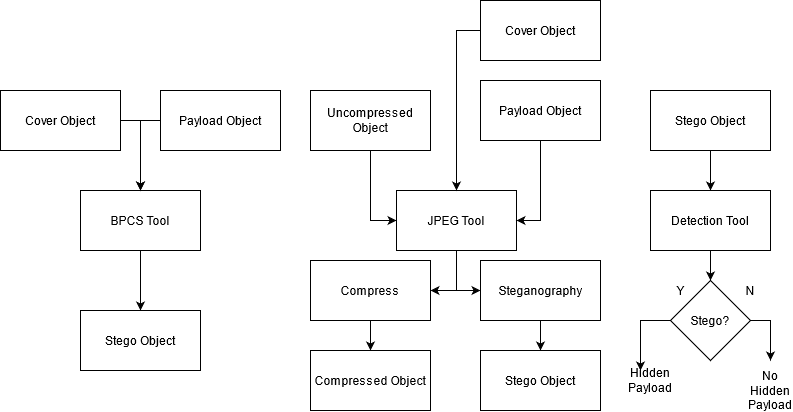
\includegraphics[width=1.0\linewidth]{images/system_architecture.png}    
    \caption{High-Level System Architecture}
    \label{fig:hlsa} 
\end{figure}

Each component is responsible for separate tasks. Although, depending on a user's desired workflow, sequential use is suitable. As an example, the BPCS tool will take cover and payload objects to produce a stego object. Following this, the stego object can then serve as input for the detection tool.

\section{BPCS Tool} \label{bpcs_design}

Delving into the BPCS tool and its encoder and decoder child components, the former takes in cover and payload objects and subsequently converts them to gray coding. A bit-plane array is created for each object and divided into 8x8 blocks. We replace the complex blocks in the cover with payload blocks, conjugating if necessary. We store a conjugation map maintaining a record of conjugated blocks and payload metadata detailing the payload dimensions and the total number of embedded blocks. After completion, we convert back from gray coding to produce the stego object. The decoder process is the encoder steps in reverse. This design is visualised in figure \textbf{\ref{fig:hlsa_bpcs}}.

\begin{figure}[]
    \centering
    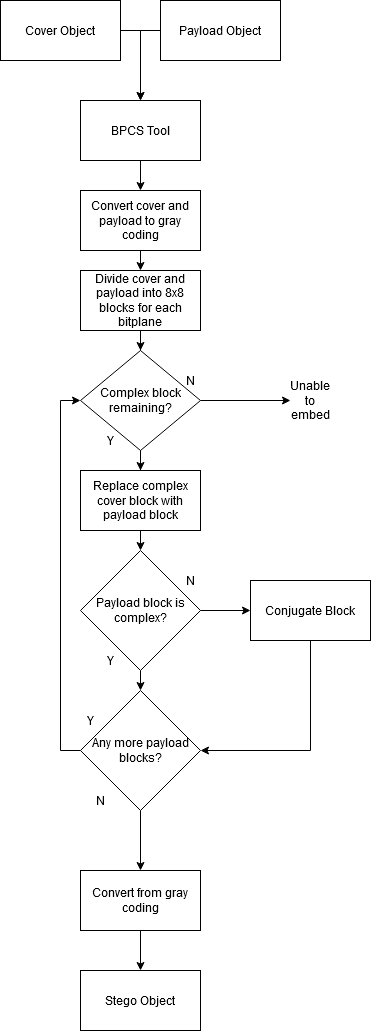
\includegraphics[width=0.6\linewidth]{images/bpcs_architecture.png}    
    \caption{High-Level System Architecture of BPCS Tool}
    \label{fig:hlsa_bpcs} 
\end{figure}

\subsection{Modifications}\label{modifications_design}

Alternatively, in the BPCS tool, a user can select the modified algorithm. The steps in this are the same as those in the standard algorithm, albeit with two modifications. Our two modifications are as follows: "variable complexity" and "random bitplane embedding order". Regarding the former, we define it as different embedding thresholds for each of the eight image bitplanes. Contrastly, a single static complexity measure exists using the standard algorithm. Modification values are between the range of 0 and 0.45. Secondly, we define random bitplane embedding order. Standardly, payload blocks are taken sequentially and embedded in the cover object, starting with the LSB to the MSB bitplane.  In our modification, we instead replace the bitplane embedding order with a randomised one. A pseudo-random number generator facilitates this by using the cover object height as a seed value.

Recall the steganalysis technique discussed in section \textbf{\ref{steganalysis}}, where a "valley-like" signature indicates BPCS embedding. Our modifications address this vulnerability in two ways. Firstly, variable complexity alters the position of the valley in each bitplane. Secondly, bitplane embedding order further ensures reduced consistency in which bitplane the valley occurs. With the standard algorithm, every stego object will contain a valley signature in the same bitplane since the embedding order is constant. By changing the order, we ensure that no consistent pattern in valley signatures appears, meaning any other secret communication is left uncompromised in the event of suspicion raised against one stego image.

\section{JPEG Tool}\label{jpeg_design}

\subsection{JPEG Compression}

JPEG compression is performed solely in the encoder component of the JPEG tool. Design of compression per the baseline JPEG standard discussed in section \textbf{\ref{jpeg_overview}}. We take an uncompressed image, split it into 8x8 blocks, perform the Discrete Cosine transform on each block, normalise with the quantization matrix, perform zigzag encoding and then run-length encoding. Following this, the compressed image is created by performing these steps in reverse order. The high-level design of the compression functionality of the JPEG tool can be seen in figure \textbf{\ref{fig:hlsa_jpeg_compress}}.

\begin{figure}[]
    \centering
    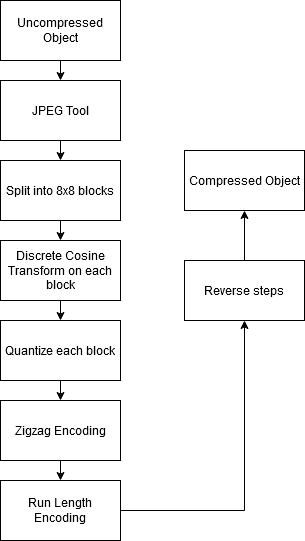
\includegraphics[width=0.5\linewidth]{images/jpeg_compression_architecture.png}    
    \caption{High-Level System Architecture of JPEG Tool (Compression)}
    \label{fig:hlsa_jpeg_compress} 
\end{figure}

\subsection{JPEG Steganography}

Both the encoder and decoder components of the JPEG tool are responsible for performing JPEG steganography. Method of data hiding through using a spatial domain steganographic technique such as LSB embedding. Crucially, the embedding process must take place after compression or the data is lost. Thus, rendering the payload unrecoverable. Tying this description to an architectural diagram, we have figure \textbf{\ref{fig:hlsa_jpeg_steg}}.

\begin{figure}[]
    \centering
    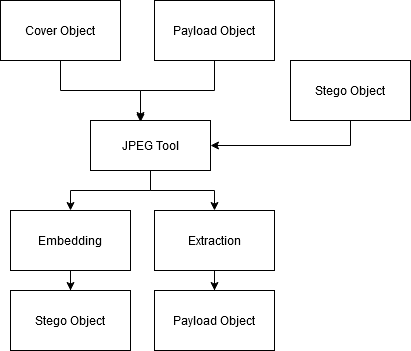
\includegraphics[width=0.6\linewidth]{images/jpeg_steganography_architecture.png}    
    \caption{High-Level System Architecture of JPEG Tool (Steganography)}
    \label{fig:hlsa_jpeg_steg} 
\end{figure}

\section{Detection Tool}\label{detection_design}

We categorise the detection of a hidden payload into four detection cases in the tool. These are a known cover and stego, known payload and stego, known algorithm and stego, and stego object only. The more information we can supply to the tool, the higher the likelihood of successful detection, which reduces false positives and false negatives. Each of the cases form part of the architecture displayed in figure \textbf{\ref{fig:hlsa_detection_tool}}.

We outline the core way each detection case functions. For a known cover and stego, perform a simple comparison. If these are not equal, then hidden data is present. For a known payload and stego, split each image into 8x8 blocks and check that each payload block exists in the stego. For a known algorithm and stego, check the first complex block if the values extracted make sense as metadata; then there is a hidden payload. Lastly, the stego object should automate the manual check for the "valley-like" signature in the complexity histogram.

\begin{figure}[]
    \centering
    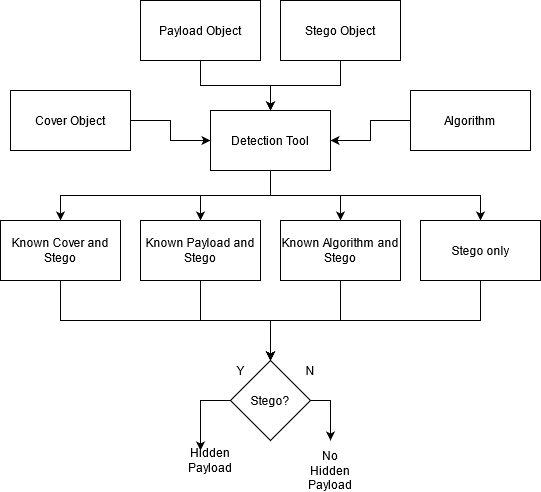
\includegraphics[width=0.8\linewidth]{images/detection_tool_architecture.png}    
    \caption{High-Level System Architecture of Detection Tool}
    \label{fig:hlsa_detection_tool} 
\end{figure}

\section{Summary} 

This chapter presented the high-level design of the developed system. Such a design included the broader architecture, further broken down into the individual components of the system. Coupled with a description of the BPCS algorithm modifications was a justification for why each would positively address the identified vulnerability. An overview of the cases involved in the detection tool concluded the work in the chapter.

%==================================================================================================================================
\chapter{Implementation}\label{Implementation}

This chapter details the steps taken in implementing the system based on the high-level design discussed in section \textbf{\ref{Design}}. Topics covered include development strategies, unexpected changes, and libraries/language/frameworks used. Centrally, we describe the specific implementation achievements relating to each system component.

\section{Version Control}

Version control \citep{version_control} was of critical importance to manage project progression. Due to potential integration with issue tracking systems, Github prevailed as the choice of platform. The development life-cycle revolved around a trunk-based branching strategy. A clean master branch, coupled with a working development branch, ensured a degree of separation. Meaning any issues that arose when working on one part of the system could be reverted, with no effect on previously completed features. "Releases" would occur in the form of merging to master to reflect the achievement of particular milestones, e.g. a single working modification to the BPCS algorithm.

\section{Development Methodology}\label{development_methodology}

Quickly into development, a feature-driven approach emerged as more suitable and sustainable than the initially chosen test-driven development approach. Kanban is a simple and popular framework that facilities this methodology. In Kanban, "Work items are represented visually on a Kanban board, allowing team members to see the state of every piece of work at any time." \citep{kanban}. Section \textbf{\ref{issue_tracking}} describes this board in further detail. Work items from the backlog were chosen and developed throughout a one-week sprint \citep{sprints}. Feedback from the supervisor meeting would shape the selection of work items for the subsequent sprint.

\section{Issue Tracking and Time Management} \label{issue_tracking}

Trello \citep{trello} is a web-based issue tracking service that allows teams to use particular frameworks, including a Kanban board, in their workspaces. Trello allowed for categorising work items into their respective system component - BPCS, JPEG or DETECTION. Additional colour coded tags such as - "bug", "refactoring", or "feature" - could be added to provide further information about each issue. Trello boards were an invaluable addition to see an overview of the current state of the project. Additionally, timelines of planned project progression, taking the form of a Gantt chart, were created each semester. Proper time management maximised productivity by focusing on the high-value items in the list of prioritised requirements.

\section{Development Language}

Python \citep{python} is the development language of choice for the project. One key factor considered was the availability of existing libraries for image processing and numerical operations. Section \textbf{\ref{Libraries}} discusses the used python libraries in depth. Since python syntax is much like pseudo-code, the implementation process will be intuitive, ensuring that the only learning curve during development will be with the project content, not the language itself. That is beneficial in the event of another developer carrying on with the project based on specified future work - it will be easier to understand the code-base.

\section{Libraries Used}\label{Libraries}

\subsection{Pillow}\label{pillow}

Pillow \citep{pillow}, known by the shorthand PIL, is an image processing library for Python. Pillow provides support for reading and writing images in a variety of formats. That is especially useful given we will be working with both .bmp and .jpg images. Despite being a more general library, PIL is more suitable than other alternatives like sci-kit, as our instances of image processing are relatively simple tasks.

\subsection{OpenCV-Python}\label{opencv}

During the development of the JPEG tool, issues arose -  discussed in detail in section \textbf{\ref{joeg_steganography_implementation}} - when implementing the Discrete Cosine Transform (DCT) and Inverse Discrete Cosine Transform (IDCT) of image blocks. The OpenCV \citep{opencv} library provides built-in functionality for these operations. However, the OpenCV DCT and IDCT required OpenCV objects. Consequently, OpenCV also handles image file reading.

\subsection{Numpy}

"NumPy is the fundamental package for scientific computing in Python" \citep{numpy}. Numpy itself is not a required package for solving the aims of the project. However, it is crucial if we want to make the system usable. Numpy provides multidimensional array objects. These are significantly faster than standard array objects during computations such as shape manipulation, sorting, logical and mathematical operations. Numpy's inclusion is responsible for the faster performance of each tool in the system.

\subsection{Argparse}\label{argparse}

Each component of the system will be a command-line application. This is discussed in further detail in section \textbf{\ref{command_line}}. Argparse \citep{argparse} makes these command-line applications more user-friendly by providing help, usage and error messages when parsing user arguments. Argparse allows for both optional and positional arguments. The former is useful in the detection tool as a variable number of arguments will be provided. The latter is useful in the BPCS tool, which requires a set number of arguments.

\subsection{Plotly}

Plotly \citep{plotly} is a graphing library for Python providing the ability to generate multiple kinds of visualisations.  These include but are not limited to scatter plots, bar charts and distribution plots. Of particular use were distribution plots that visualise a probability distribution of block complexity measures. Plotly was needed for an initial manual inspection to determine whether the evaluation process should use the planned steganalysis techniques.

\subsection{Sphinx}\label{sphinx}

Sphinx is a library used for generating HTML directly from code comments. Extensive documentation promotes the maintainability and extensibility of the project. Sphinx features include "syntax highlighting, searchable index, module index, document tree, hierarchical structure and extensive cross-referencing" \citep{sphinx}. The HTML also includes installation notes which give an overview of how users can get a local version running on their system.

\section{User Interface}

Bearing consistency in mind when designing a user interface is crucial.  Ensuring that each component in the system's design reflects a design standard promotes increased system usability. Differing tool design would lead to users feeling overwhelmed and put off from using the system \citep{consistency}. 

\subsection{Command Line Application} \label{command_line}

The implemented system need only contain functionality that meets the previously prioritised list of requirements. A command-line application best suits this, and changing this to a different form of application does not offer extra utility. We have to account for parameterisation. "Most operating systems support a means to pass additional information to a program when it is launched." \citep{commandline}.  Following simple input from the user, the application takes care of the rest. Users are assumed to have sufficient technical experience. However, the help parameters can be used at any time to view instructions on using the system. Each command-line application can work in combination as part of a user workflow. Alternatively, they can work independently to promote modularity. Additionally, as each component is self-contained, further extensions to the project do not require significant changes to the underlying architecture.

\section{BPCS Tool}\label{implementation_bpcs_tool}

Implementation of the BPCS tool followed the high-level design specified in section \textbf{\ref{bpcs_design}}. Initially, the implementation of the standard algorithm preceded the development of two modifications. The BPCS module contains two separate python files, encode and decode, to perform embedding and extraction operations.  As justified in section \textbf{\ref{command_line}}, users interact with the tool through a command-line application. Parameters in the form of the cover image, payload image, and algorithm selection are required for the tool to function. We use the Argparse library, overviewed in section \textbf{\ref{argparse}} to facilitate this. Argparse positional arguments ensure that an error message is displayed if any of the specified parameters are missing. Additionally, we restrict the algorithm parameter to a selection from a predefined list of acceptable choices. Listing \textbf{\ref{lst:argparse_bpcs}} shows the source code for command-line argument parsing in the BPCS tool. 

\begin{lstlisting}[language=python, float, caption={Command-line argument parsing using the Argparse library. Cover, payload and algorithm selection specified as positional arguments. Algorithm selection restricted to a choice from a set of predefined options.}, label=lst:argparse_bpcs]
    def get_arguments():
    parser = argparse.ArgumentParser(description="BPCS Encoding tool")
    parser.add_argument("v", type=str, help="Cover Image")
    parser.add_argument("s", type=str, help="Payload Image")
    parser.add_argument("a", choices=["standard", "improved"], type=str, help="Algorithm. Standard or Improved")
    args = parser.parse_args()
    return args
\end{lstlisting}

After parsing user arguments, the Pillow library discussed in section \textbf{\ref{pillow}} reads the relevant images. Each image read is now a Pillow Image object containing predefined methods that we can use. One such example of this is the "mode" method. "Mode" returns particular flags to indicate the colour depth of an image. Flags "L" and "P" reflect an 8-bit colour image. Flag "RGB" reflects a 24-bit colour image. Two helper functions allow for different behaviour based on the image mode. The get\_grayscale\_channel helper returns a single element list where the element is the single channel in an 8-bit colour image. The get\_colour\_channels helper returns a list of length three, where elements are the individual channels in an RGB 24-bit colour image.

Using an adapted online implementation \citep{gray-code-conversion}, we convert each channel in both the cover and payload from binary representation to the respective gray coding representation. The operation is suitable for vectorization to significantly increase speed as it takes a NumPy array object as a parameter.  For a given value x, to convert to gray coding, we take the Logical XOR operation of x and y, where y is the x value right-shifted by 1 bit. In python, the right-shift operator is ">>". Right-shifting by 1 is simply "chopping off" the least significant bit and placing a 0 at the front of what remains. Example illustration of Right-shifting:

We have the value 16, where its binary representation is 00010000. We "chop off" the least significant bit, i.e. 0 to produce 0001000. Placing a 0 at the front of what remains leaves us with 00001000. Deriving from the logical XOR of 00010000 (x) and 00001000 (y), 16 in gray coding is 00011000. 

Unfortunately, during gray coding to binary conversion, we do not benefit from vectorization as we had done previously. Every value in the NumPy matrix experiences the following operation. For a given value x, to convert to binary, we take the Logical XOR of the inverse (where the inverse initially starts at 0) and value x. After, x is then right-shifted by one. The new value of inverse is the result of the logical XOR. The steps repeat until the value of x is zero. 

Dependent upon the user selection of the embedding algorithm, chosen complexity thresholds will vary. In the standard algorithm, each bitplane has the same threshold measure. Whereas with the modified algorithm, the values range between 0 and 0.45. A dictionary mapping algorithm choices as keys to a list of embedding thresholds is indexable with the parsed user parameter. 

Consider the list [7,6,5,4,3,2,1,0] - the standard bitplane embedding order of the BPCS algorithm. Reshuffling of this order will occur when using the modified algorithm. Accomplishing this requires the "shuffle" function from the python "random" library \citep{random}. Shuffle takes a seed value to produce a reordered list. This order must stay consistent for embedding and extraction if we aim to recover our hidden payload. Hence, we use the height of the first channel in the image as a seed. Splitting each image into 8x8 blocks for each bitplane, we create 3-Dimensional NumPy bitplane arrays of shape (m,n,8) - m and n in this context represent the height and width of the image.


Payload metadata is similarly embedded to ensure a successful extraction can take place. This metadata exists as the first complex 9x9 block in the cover object by setting rows to values. Rows one to four of the block represent the total number of payload blocks. Rows five and six are the height of the payload object.  Following this, rows seven and eight are the width of the payload object. The remaining row is 0s. 

Once these preliminary tasks have finished, we begin the main body of embedding work. Consider three scenarios of BPCS tool usage. If embedding an 8-bit colour payload image in an 8-bit colour cover image, we embed the single payload channel in the other single cover channel. Alternatively, with the same payload and a 24-bit colour cover object, we embed the single payload channel within the red channel of the cover. Finally, each colour channel is embedded within the twin colour channel if both the payload and cover are 24-bit colour images. Now the steps of embedding. Metadata is first embedded. We loop through each block in the cover and replace it with a payload block if complex. List of payload blocks act as a queue and are popped from the queue once embedded in FIFO order (First In First Off). Non-complex blocks, if necessary, are conjugated using the conjugation operation.  The program will exit if the number of still-to-be-embedded payload blocks exceeds the remaining capacity of the cover. As a means of storing the conjugation map, we use 9x9 blocks during embedding. There must be some way of knowing which blocks were conjugated. To do this, we set the 9th row, 9th column value to 1 to indicate a conjugated block and to 0 for non-conjugated. We embed payload data in the 8x8 region of the 9x9 block. After embedding has taken place, the resulting gray coding to binary representation conversion of the stego image is then written to disk using the Pillow library. 

BPCS decoder takes images and converts them to gray coding representation, returning a list of channels in the same fashion as the encoder. As opposed to splitting into 8x8 blocks, we instead split into complex 9x9s. Set of complexity thresholds taken from the dictionary indexed by algorithm selection. Since the decoder performs the previous steps in the BPCS encoder in reverse order, it is redundant to cover some aspects of the extraction process. Instead, we will highlight areas of interest. Listing \textbf{\ref{lst:metadata_extract}} shows the process of metadata extraction. When extracting metadata, the NumPy ravel function \citep{ravel} allows us to flatten the desired rows into a single array. Note that extraction raises a memory error if the recovered height is greater than the current stego object's height. Any discrepancy here indicates that the algorithm selected during the decoding phase is different from the one used to embed. Continue extracting complex blocks and take 8x8 region from them until the extracted number of blocks equals the total block count recovered in metadata. An 8x8 block either is or is not conjugated based on the 9th-row 9th-column value. Recall this is how we store the conjugation map during embedding. A value of 1 indicates conjugation. A value of 0 entails that the block is not conjugated. Reconstruct image using the height and width from metadata.

\begin{lstlisting}[language=python, float, caption={Extraction of metadata by the BPCS tool decoder component}, label=lst:metadata_extract]
    def extract_meta_data(payload, stego_arr):
        meta_data = payload[0]  
        payload.pop(0)
        if meta_data[8,8] == 1:
            meta_data = conjugate(meta_data)
            meta_data[8,8]=0
            
        total_blocks = np.ravel(meta_data[:4,:])
        height = np.ravel(meta_data[4:6,:])
        width = np.ravel(meta_data[6:8,:])
        
        total_blocks = int("".join(str(elem) for elem in total_blocks), 2)
        height = int("".join(str(elem) for elem in height), 2)
        width = int("".join(str(elem) for elem in width), 2)
        if (height>stego_arr.shape[0]):
            raise MemoryError("Wrong algorithm used for decoding")
        return (total_blocks, height, width)
\end{lstlisting}

\section{JPEG Tool}\label{jpeg_implementation}

The JPEG tool is the system component responsible for performing JPEG compression and JPEG steganography. Implementation followed the high-level design outlined in section \textbf{\ref{jpeg_design}}. 

\subsection{Compression}

Users interact with the JPEG tool through the command line application. Arguments passed to the program are parsed using the Argparse library. These arguments come in the form of an uncompressed image, payload image, and algorithm choice - this choice can be compression or any of the implemented forms of steganography. The latter argument is specified as a positional argument, whereas the other two are optional arguments. Standard chrominance and luminance quantization tables, seen in table \textbf{\ref{q_matrices}}, were sourced from \citet{attaby_2021}. Multidimensional NumPy array objects represent each matrix. Additionally, each matrix is a global variable, meaning any function can use it without repeatedly passing it as a parameter.

Using the OpenCV library, we first read the appropriate images. If the user selects "compression" for the algorithm choice parameter, we ignore the payload image. Much like the Pillow library, OpenCV allows us to check the colour depth of an image. The "shape" of an OpenCV image object is akin to Pillow's "mode" function. A shape of length 2 indicates an 8-bit colour image, with any other value being a 24-bit colour image. Based on the colour depth, we reperform image reading with the addition of one of two flags. Flag "IMREAD\_GRAYSCALE" will read the image in 8-bit colour. Flag "IMREAD\_RGB2YCrCB " will read in the 24-bit colour image. Recall that JPEG compression works with a particular colour space. Hence, for a 24-bit colour image, conversion between RGB and YCbCr colour spaces occurs. Resizing of image dimensions is performed to be divisible by 8. 

The core functionality of the algorithm resides in a single function. Firstly, we create a row in a CSV file. This row is the height and width of the uncompressed image. After splitting the image into 8x8 blocks, we loop through each block and perform the discrete cosine transform using the built-in OpenCV function. As expressed previously, this was the foremost benefit of OpenCV and replaced a previous implementation using the SciPy library. The following formula shows the alternative DCT operation using SciPy.

\begin{verbatim}
dct(dct(a.T, norm='ortho').T, norm='ortho')
\end{verbatim}


Breaking this formula down, we perform the DCT operation on the transposed matrix of the DCT operation on the transposed matrix. What this involves is that the DCT is first performed column-wise and then row-wise. Next, we normalise the block with the respective quantization matrix - chrominance or luminance. An existing online implementation of zig-zag encoding \citep{lfv-compression} then reorders the resulting DCT coefficients.

The previously created CSV file is updated to include the run-length encoding (RLE) of each block. Python's "itertools" library contains the "groupby" function. Groupby, seen in listing \textbf{\ref{lst:rle_itertools}}, lets us group consecutive occurrences of elements. Illustrating with an example: ("AAABCDD") would become ["A", "A", "A"], ["B"], ["C"], ["D", "D"]. A group value and count of elements in the group is appended to a list of lists. For the first group in the previous example, this would result in [["A", 3]]. In turn, we add this as a new row in the CSV file.

\begin{lstlisting}[language=python, float, caption={Creation of Run-Length Encoding using Python's itertools library.}, label=lst:rle_itertools]
    rle = [[i, len([*group])] for i, group in groupby(block)]
\end{lstlisting}

To reconstruct a block, we read a row from the CSV file. However, this presents a problem. As each row is a String, we are unable to index the list. We can evaluate the String to a python type using the python "ast" library \citep{ast}.  We multiply the value by the count in each list to create a 1-Dimensional NumPy array object. Inverse zig-zag encoding takes a 64 element 1-D list to produce an 8x8 block. The remaining steps are to multiply the block with the quantization table, perform inverse discrete cosine transform and create the new image using the OpenCV "imwrite" function.

\subsection{Steganography}\label{joeg_steganography_implementation}

Our approach to JPEG steganography encompassed three spatial domain techniques. These were: LSB steganography, Third LSB steganography and random order Third LSB steganography. Each is a variation of one another as all operate based on a simple substitution of cover data for payload data. Despite planning only to implement LSB steganography, the use of the OpenCV library presented a problem. Two mechanisms facilitate the creation of an image. Either spend a substantial portion of time creating a novel encoder; this would involve working with byte arrays and manually specifying image headers. Or we can use the OpenCV "imwrite" function to take an array and produce an image from it. A clear choice emerged from these two possibilities. However, it came with unintended consequences.  When we specify that we want a .jpg to be created by "imwrite", we are asking it, in effect, to perform all the compression steps previously implemented, resulting in a double compression. Recompression produces an image different from expectation. Consider this in the context of steganography; simple substitution techniques are not robust enough to survive compression.  That is why the embedding must take place after the compression process. We can mitigate the problem of this recompression, to a certain extent, by setting the "imwrite" JPEG\-QUALITY factor to 100. A value of 100 is the minimum amount of compression possible. Despite this, we still end up with variances of +1 and -1 in the actual and expected pixel values. These differences will be reflected in the LSB, rendering the payload unrecoverable when using the LSB technique.

Note that these variances are of value at most 1, meaning we can intentionally restrict this phenomenon to only affect the LSB and 2nd LSB. Herein lies the motivation for 3rd LSB. 3rd LSB operates in the same way as LSB, only in a different bitplane. How does this mitigate the problem of variance? Illustrating with an example: Let's say our expected binary representation of a pixel is 11110000. We embed 1 in the 3rd LSB and set  LSB to 1, resulting in 11110101. +1 change will result in 11110110, while -1 will result in 11110100. In each case, only the 1st and 2nd LSB are affected. As a result, we can safely embed in the 3rd LSB without fear of losing the payload due to recompression. 

Random order 3rd LSB makes one modification to the 3rd LSB technique. As opposed to traversing every pixel sequentially, we perform a random selection from the image, 8 pixels at a time. Functionality exists in the form of the "sample" function from the python "random" library \citep{random}. Cover image height is chosen as the seed value to ensure the pseudo-random order is consistent for embedding and extraction. 

\section{Detection Tool}\label{implementation_detection_tool}

Implementation of the detection tool followed the high level design specified in section \textbf{\ref{detection_design}}. Like the BPCS and JPEG modules, users interact with the tool using the command-line. 

Crucially, the more parameters a user can provide, the higher the likelihood of successful detection. All possibilities of user-specified detection cases are mapped to functions in the source file using a dictionary. Presenting each of these cases in order of highest to the lowest likelihood of successful detection: known cover object and stego, known payload and stego, known algorithm and stego, and finally stego object only. After parsing user arguments using the Argparse library, we index the function\_call dictionary to execute the appropriate function. Code from the BPCS module, such as reading files using Pillow, splitting into 8x8 blocks, and calculating complexity measures, is imported rather than rewritten to eliminate code redundancy. Listing \textbf{\ref{lst:detection_tool_dict}} shows the source code of the implemented dictionary and function execution - detection case parameter is a number, not a string, to save the user typing out the case each time.

\begin{figure}[!h]
    \centering
    \begin{subfigure}[b]{0.85\textwidth}
        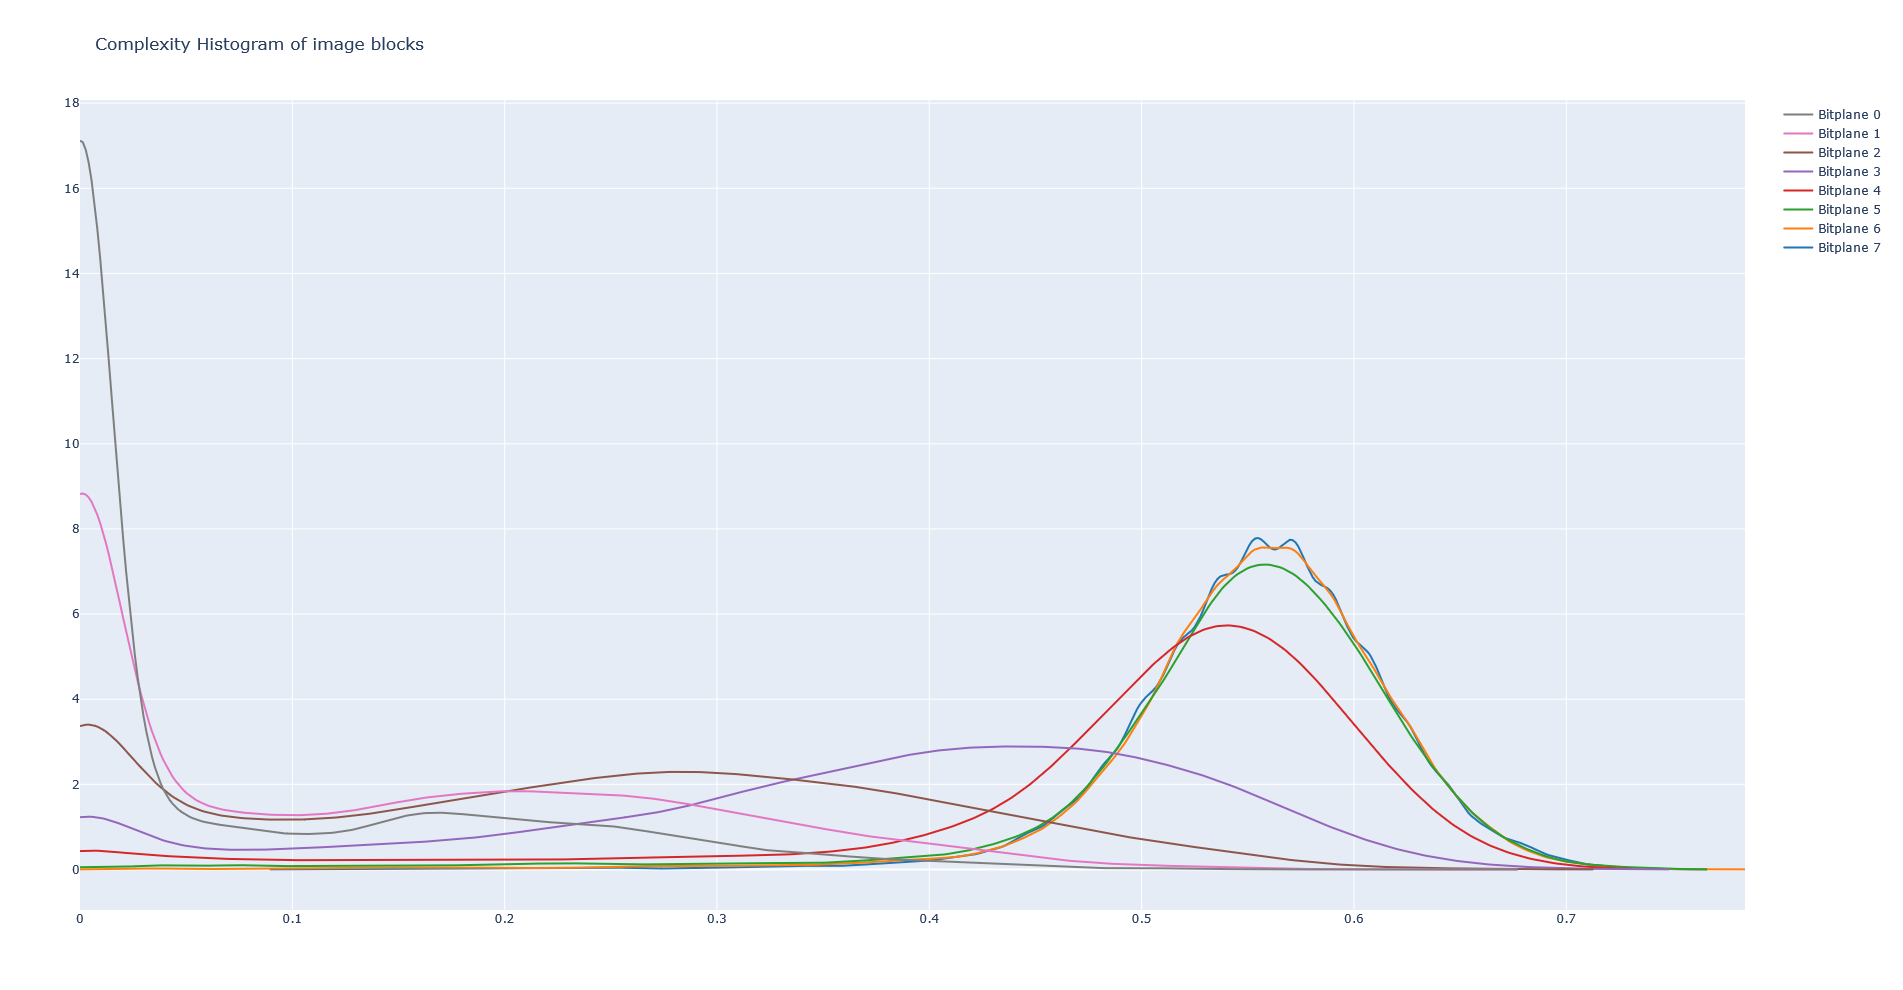
\includegraphics[width=\textwidth]{images/natural_no_vuln.png}
        \caption{Natural image "vessel.bmp" with no vulnerability. Block complexities do not exceed threshold in detection case.}
        \label{fig:natural_no_vuln}
    \end{subfigure}
    \begin{subfigure}[b]{0.85\textwidth}
        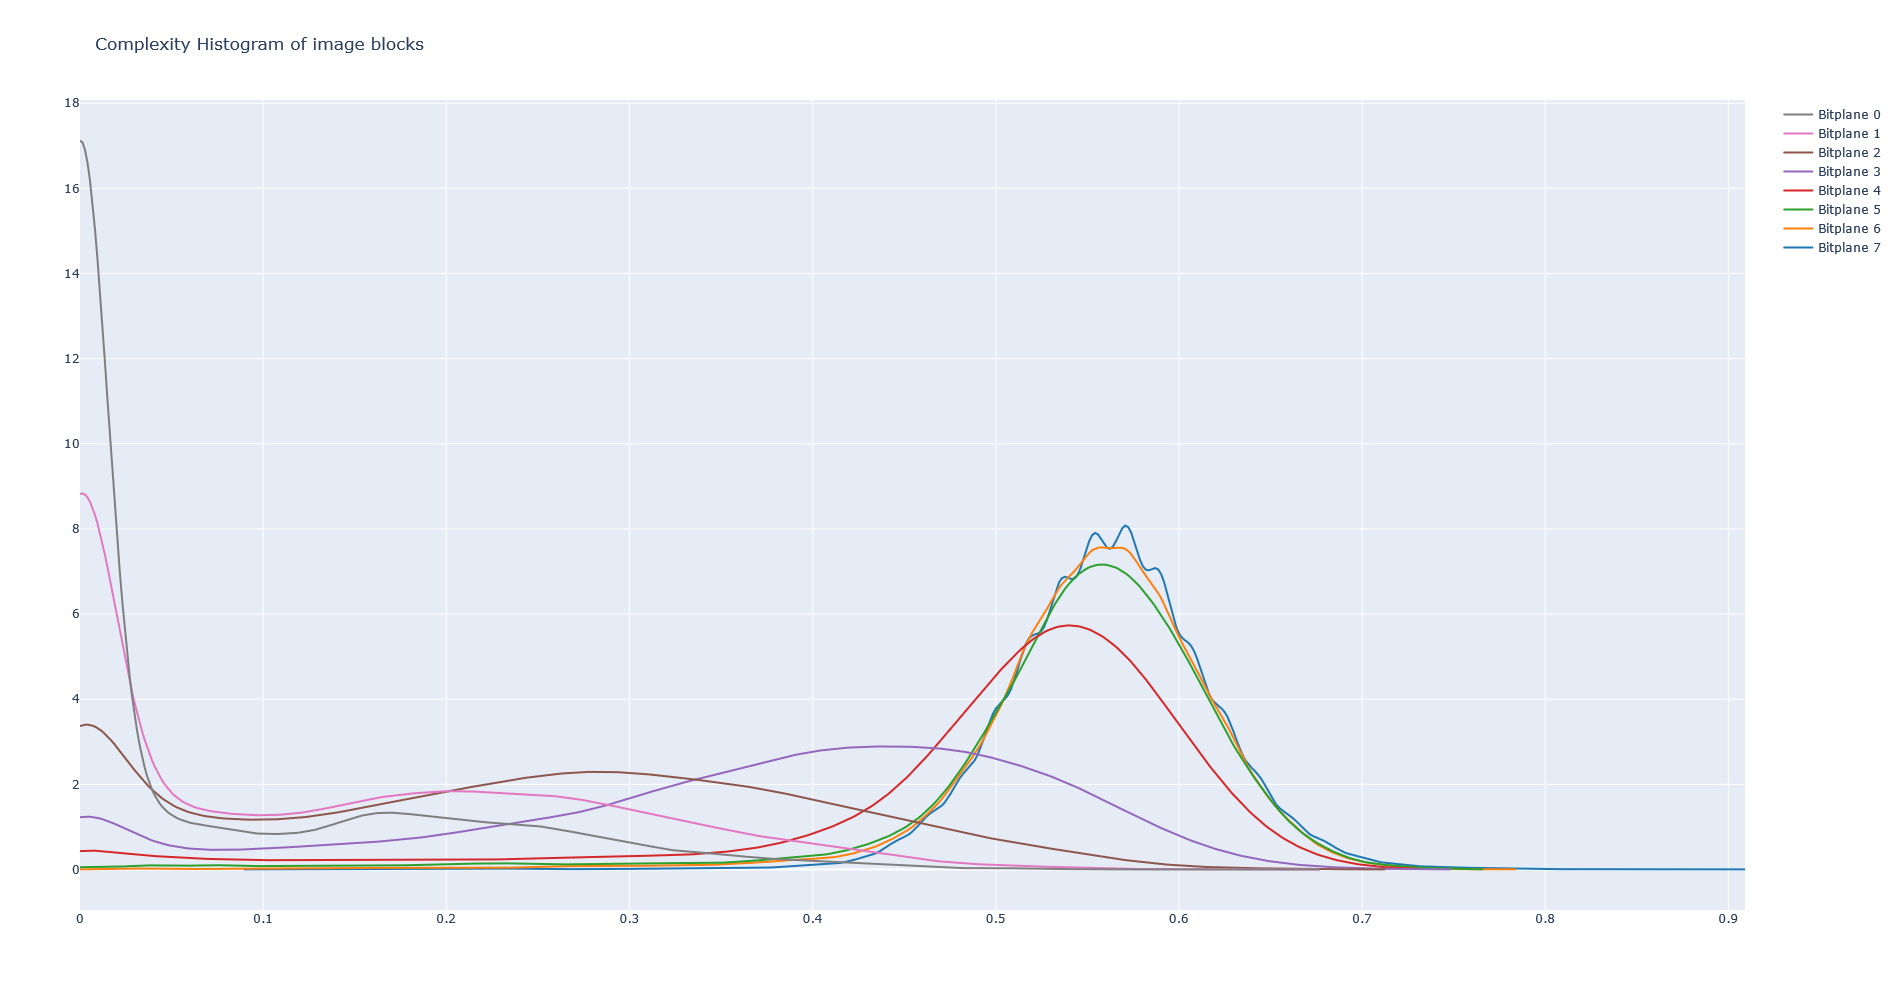
\includegraphics[width=\textwidth]{images/stego_vuln.png}
        \caption{Stego image "stego.bmp", made from "secret.bmp" embedded in "vessel.bmp", with the vulnerability. Block complexities exceed the threshold in detection case.}
        \label{fig:stego_vuln}
    \end{subfigure}
    \caption{Distribution plots of block complexities within images. The steganalysis technique used in the stego object only detection case. Figure \subref{fig:natural_no_vuln} shows the distribution plot for a natural image. Figure \subref{fig:stego_vuln} shows the distribution plot for a stego image.}
\end{figure}

In the case of a known cover object and stego, we use a straightforward comparison during detection. Each image is read using Pillow and represented as a NumPy array object. Using the "==" operator gives an ambiguous result as there is more than one value in each array. Due to this, we specify that every element is subject to the comparison using the numpy.all() \citep{all} function. If equal, then the suspected stego object is said to be clean. Otherwise, there is a hidden payload present. 

In the case of a known payload and stego object, we again use a simple comparison, albeit with an additional preliminary step. We split the stego into 9x9 blocks and the payload into 8x8 blocks. Next, we have a two-stage comparison process. Firstly we compare a payload block with the 8x8 region of a 9x9 block in the stego. Secondly, we compare the conjugated versions of these payload and stego blocks. A hidden payload exists should a match be found in either pass, else the suspected stego is clean.

\begin{lstlisting}[language=python, float, caption={Detection tool dictionary mapping user selected detection case to functions in the program.}, label=lst:detection_tool_dict]
    function_calls = {
        0: known_cover_and_stego,
        1: known_algorithm_and_stego,
        2: known_payload_and_stego,
        3: stego_only
    }
    function_calls[mode](args)
\end{lstlisting}


Metadata describing the payload must persist after embedding so that the decoder can reconstruct the image.  Regardless of the embedding algorithm used, metadata values are subject to some of the same restrictions. The height and width of an embedded payload cannot be greater than those of the cover object. This condition is integral to the detection case of a known algorithm and stego. We borrow functionality from the BPCS decoder and attempt metadata extraction. Should the previously mentioned condition be violated, the decoder raises a MemoryError. Exception handling in the detection tool then allows us to determine the presence of a hidden payload. A caught exception indicates that the extracted height and width is greater than the cover image dimensions, thus violating the condition. Hence, the suspected stego is clean. Otherwise, a hidden payload is present.

Section \textbf{\ref{steganalysis}} outlined the planned steganalysis technique for the case of a stego object only. However, this implementation could not reproduce the valley signature, and the absence of it was verified by investigating distribution plots created using the plotly library. Repeated analysis of the image histograms paved the way to devise a backup technique and subsequent development. Block complexities greater than 0.9 are consistent in stego images where embedding has taken place using BPCS as seen in figure \textbf{\ref{fig:stego_vuln}}. They are not present in natural images as seen in figure \textbf{\ref{fig:natural_no_vuln}}. BPCS conjugation serves as a potential explanation of this effect. Consider the embedding of a block with complexity 0.05 in a suitable cover object. This block does not meet the chosen complexity threshold and must be conjugated to assign a new value of (1-x), where x is the original complexity measure, giving 0.95.  As these high complexity blocks do not exist in natural images, a manual inspection of the histogram with this in mind highlights BPCS embedding. Digital detection can then be performed by creating an array of block complexities and taking the maximum value. If this maximum value exceeds our chosen threshold of 0.9, then a hidden payload is present. Otherwise, the suspected stego object is clean.

\section{Summary}

This chapter described the implementation of the system. Part of this process involved identifying external libraries, and development practices like version control and issue tracking. Justifications for such choices served as preliminary work for the specific implementation details of core functionality in each system component. Problems that arose were mitigated with the introduction of a new steganalysis technique to facilitate future evaluation.
 
%==================================================================================================================================
\chapter{Evaluation} 

This chapter presents the evaluation of the system. A systematic approach to experimentation and some forms of automation through scripts allows for better reproducibility of results. Evaluation includes unit testing, external participation and internal validation of the requirements specified at the start of the project. 
 

\section{Unit Testing}\label{unit_testing}

Unit tests, developed with the pytest framework \citep{pytest}, are used to determine that the implementation behaves per expectation.  Example testing may be the conjugation operation or gray coding conversion in the BPCS tool. Furthermore, the coverage library \citep{coverage} produces an overview of the percentage of code reached by the test suite in the form of easy-to-read HTML. Due to the switch described in section \textbf{\ref{development_methodology}} from test-driven development to feature-driven, coverage values will be small. Test cases created near the start of the project life-cycle constitute the majority of the test suite. Further test case additions serve as suitable future work given its lower prioritisation compared with other requirements.

\section{Experiment Methodology}

Using test images within the file system, we systematically embed and extract a selection of images using each algorithm in the BPCS tool, where we isolate modifications for individual use.  This procedure also applies to the evaluation of JPEG steganography. A comparison of recovered payloads and original payloads employing a novel created tool determines success. Opting for a digital method rather than visual inspection will give a more accurate assessment and eliminate any bias that may be present.

Evaluation of the modifications to the BPCS algorithm is composed of two topics; visual detection and digital detection. For the former, external participants make a judgement on which images they deem to contain hidden payloads. Participants view these in a dictated randomised order to mitigate the impact of learning effects. Additionally, participants respond to a follow-up questionnaire, the intention of which is to gain an insight into their thought process. For the latter, we report on the detection rate of the created detection tool for the following categories of image: "natural images", "standard BPCS embedding", "variable complexity modification", and "random bitplane embedding order modification".

Furthermore, we perform compression on all images in the test bank using the JPEG tool. Following this, we perform calculations for relevant metrics such as the compression ratio, mean square error and peak signal to noise ratio. Lastly, we account for each detection case by supplying the appropriate parameters to the tool. Only the three remaining detection cases are of interest since the fourth is present for the BPCS algorithms comparison evaluation. 

\section{Test Images}

\citet{testimages} and google advanced image search are the two primary sources for the test bank. The former provides a standard set of images, while the latter allows us to restrict results to desired specifications such as file type, dimensions and colour depth. As a means of meeting requirements, images comprise 8-bit and 24-bit colour .bmp and .jpeg files. The inclusion of different colour depths ensures that findings can be spoken about more broadly as restrictions to only one type may limit generalisability. 

A listing of each image is as follows: vessel.bmp, secret.bmp, goldhill.bmp, harry.jpg, fruit.jpg, apple.bmp, lena.bmp. Each of the aforementioned can be seen in the figure \textbf{\ref{fig:test_images}}.


\section{BPCS}

\subsection{Standard Algorithm}\label{evaluation_standard_algorithm}

As specified in section \textbf{\ref{Analysis}}, the standard BPCS algorithm must be implemented in full, using a programming language of choice. Section \textbf{\ref{bpcs_design}} provided the high level design of the BPCS tool which was then implemented as described in section \textbf{\ref{implementation_bpcs_tool}}. Demonstrating this requirement has been met requires that our evaluation process shows the command-line application successfully perform embedding and extraction operations on a payload image within a cover object using the standard algorithm. 

Summarising the procedure, we will perform embedding and extraction using the command line application three times. Each separate instance will be with cover and payload parameters of varying colour depth. For the three cases, these will be an 8-bit colour cover and payload, a 24-bit colour cover and 8-bit colour payload and lastly, a 24-bit colour cover and payload. Figures \textbf{\ref{fig:standard_bpcs_encode_terminal}} and \textbf{\ref{fig:standard_bpcs_decoder_terminal}} show an example usage of the command line application during evaluation of the standard algorithm.

First, we attempt embedding of the 8-bit colour payload, secret.bmp, in the 8-bit colour cover, vessel.bmp, using the encoder functionality. The resulting stego object from this operation is displayed in figure \textbf{\ref{fig:stego_grayingray}}. Verifying the correctness of the algorithm requires the comparison of the extracted image with the original payload. We use the decoder functionality of the BPCS tool to extract the payload seen in figure \textbf{\ref{fig:extracted_object}}. A match is found, using the novel comparison tool, during the comparison of the extracted and original payloads, demonstrating successful embedding and extraction in the case of two 8-bit colour images.

\begin{figure}[]
    \centering
    \begin{subfigure}[b]{0.4\textwidth}
        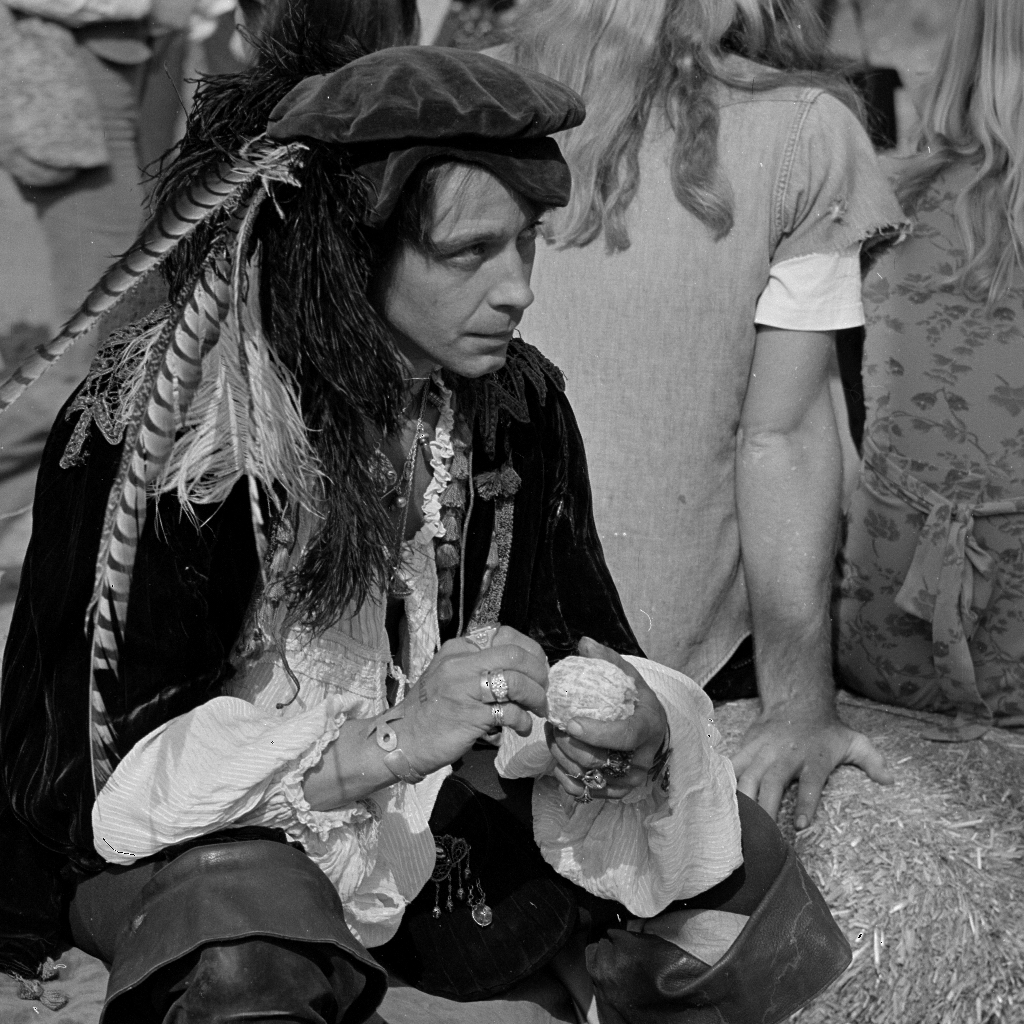
\includegraphics[width=\textwidth]{images/evaluation_grayingray_stego.png}
        \caption{Stego object produced by the embedding of secret.bmp in vessel.bmp using the standard BPCS algorithm.}
        \label{fig:stego_grayingray}
    \end{subfigure}
    \begin{subfigure}[b]{0.4\textwidth}
        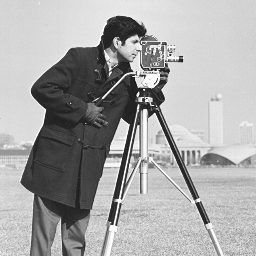
\includegraphics[width=\textwidth]{images/extracted.png}
        \caption{Payload recovered by the BPCS tool decoder.}
        \label{fig:extracted_object}
    \end{subfigure}
    \caption{Standard algorithm evaluation using an 8-bit colour payload and 8-bit colour cover. Figure \subref{fig:stego_grayingray} shows the stego object produced by the BPCS encoder from the embedding of the 8-bit colour payload, secret.bmp, in the 8-bit colour cover, vessel.bmp. Figure \subref{fig:extracted_object} shows the payload extracted by the BPCS decoder.}
\end{figure}

Similarly, we repeat this process by addressing the second case using a 24-bit colour cover object and an 8-bit colour payload. These are fruit.jpg and lena.bmp, respectively. A successful embedding using the encoder produces the stego object seen in figure \textbf{\ref{fig:stego_grayincolour}}. Following this, we use the decoder to recover the payload seen in figure \textbf{\ref{fig:extracted_lena}}. Comparing the extracted and original payloads using the novel comparison tool shows a match. Thus, demonstrating successful embedding and extraction for an 8-bit grayscale payload in a 24-bit colour cover object.

\begin{figure}[]
    \centering
    \begin{subfigure}[b]{0.4\textwidth}
        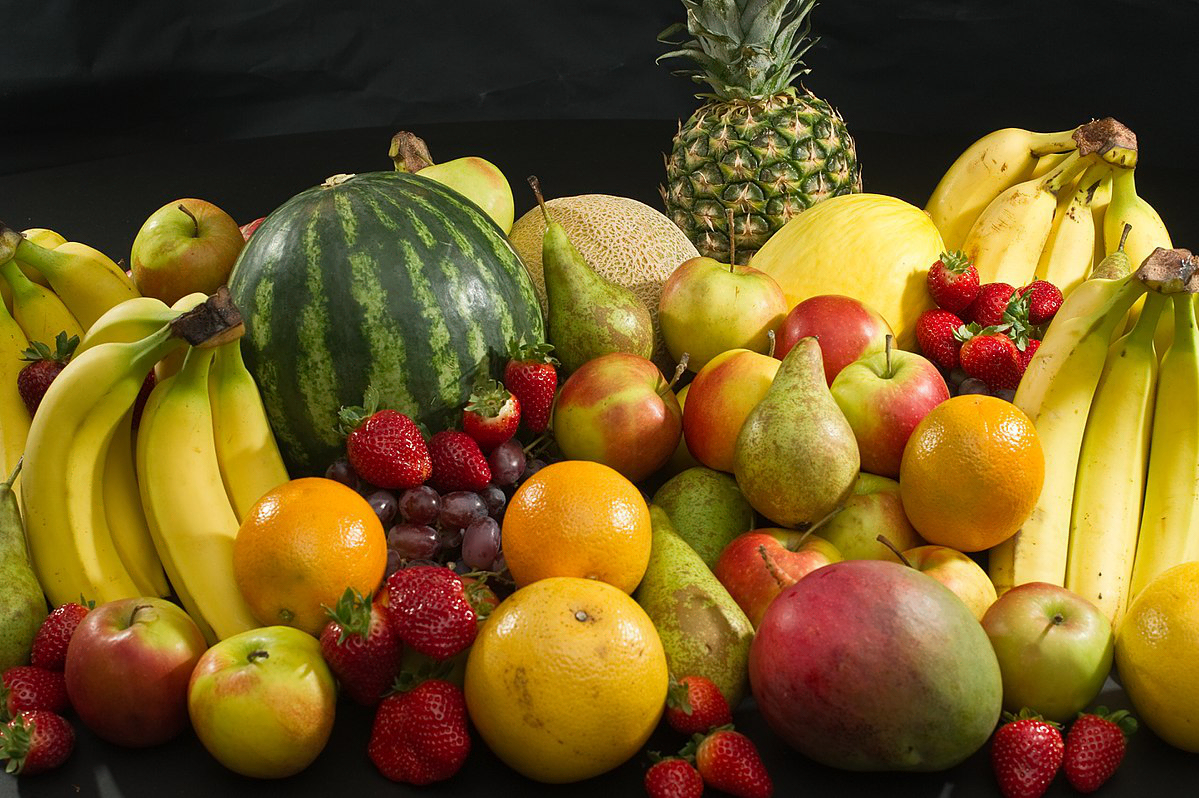
\includegraphics[width=\textwidth]{images/lena_in_fruit_stego.png}
        \caption{Stego object produced by the embedding of lena.bmp into fruit.jpg using the standard BPCS algorithm.}
        \label{fig:stego_grayincolour}
    \end{subfigure}
    \begin{subfigure}[b]{0.4\textwidth}
        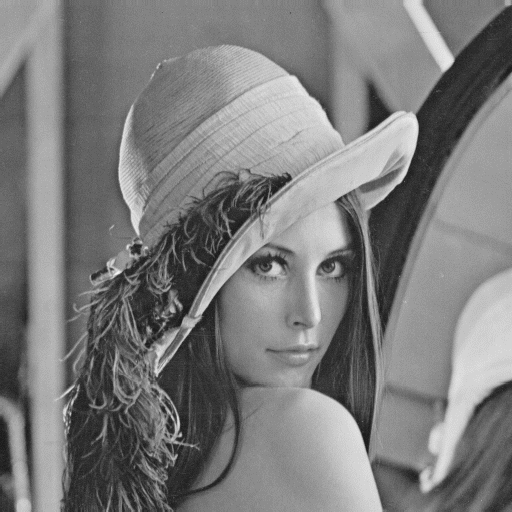
\includegraphics[width=\textwidth]{images/lena.png}
        \caption{Payload recovered by the BPCS decoder.}
        \label{fig:extracted_lena}
    \end{subfigure}
    \caption{Standard algorithm evaluation using an 8-bit colour payload and 24-bit cover. Figure \subref{fig:stego_grayincolour} shows the stego object produced by the BPCS encoder from the embedding of the 8-bit colour payload, lena.bmp, in the 24-bit cover, fruit.jpg. Figure \subref{fig:extracted_lena} shows the payload extracted by the BPCS decoder.}
\end{figure}

Lastly, addressing the case of two 24-bit colour objects. We provide parameters in the form of apple.bmp and green.bmp. Following this, we perform embedding and extraction. Figure \textbf{\ref{fig:stego_colourincolour}} shows the stego object produced by the previous process. Subsequently, the decoder recovers the payload seen in figure \textbf{\ref{fig:extracted_green}}. A comparison of the original payload green.bmp and recovered payload returns a match. Hence, demonstrating successful embedding and extraction operations for two 24-bit colour images using the standard algorithm.

\begin{figure}[]
    \centering
    \begin{subfigure}[b]{0.4\textwidth}
        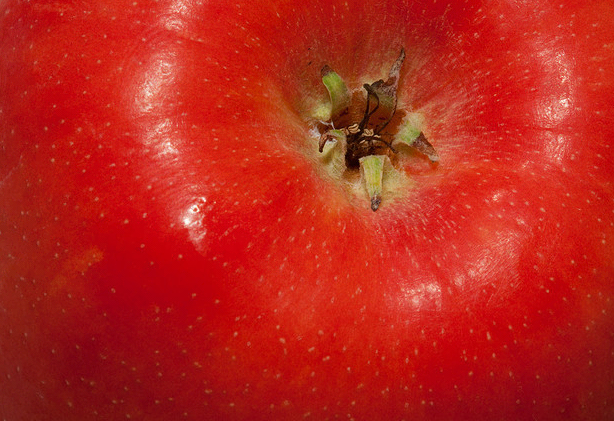
\includegraphics[width=\textwidth]{images/green_in_apple_stego.png}
        \caption{Stego object produced by the embedding of green.bmp into apple.bmp using the standard BPCS algorithm.}
        \label{fig:stego_colourincolour}
    \end{subfigure}
    \begin{subfigure}[b]{0.4\textwidth}
        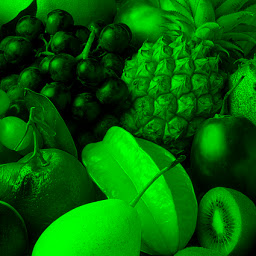
\includegraphics[width=\textwidth]{images/extracted_green.png}
        \caption{Payload recovered by the BPCS tool decoder.}
        \label{fig:extracted_green}
    \end{subfigure}
    \caption{Standard algorithm evaluation using two 24-bit colour objects. Figure \subref{fig:stego_colourincolour} shows the stego object produced by the BPCS encoder from the embedding of the 24-bit colour payload, green.bmp, in the 24-bit cover, apple.bmp. Figure \subref{fig:extracted_green} shows the payload extracted by the BPCS decoder.}
\end{figure}


The evaluation of the standard algorithm used images of varying colour depths. It was concerned with whether the BPCS tool could successfully perform both embedding and extraction operations of a payload image within a cover object. Through the previous systematic experimentation, we verified the correctness of the standard algorithm implementation. Hence, meeting the requirement.


\subsection{Modified Algorithm}\label{evaluation_modified_algorithm}

Section \textbf{\ref{Analysis}} outlines the need for modifications to the standard BPCS algorithm. Whether there is any improvement is the subject of evaluation after this section. Section \textbf{\ref{modifications_design}} provided the high level design of two modifications which were then implemented as described in section \textbf{\ref{implementation_bpcs_tool}}. Demonstrating this requirement has been met requires that our evaluation process shows the command-line application successfully perform embedding and extraction operations on a payload image within a cover object using the modified algorithm. 

The modified algorithm evaluation will follow the procedure of the standard algorithm evaluation section. Similarly, embedding and extraction using the BPCS tool take as parameter, images of varying colour depths. Additionally, these images reflect those used previously. Isolating the modifications, we have variable complexity and random bitplane embedding order.  Section \textbf{\ref{modified_use}} outlines example usage of the command line application during modified algorithm evaluation.

Addressing application usage in the case of two 8-bit colour, payload and cover images, namely secret.bmp and vessel.bmp. Using the encoder functionality for each of the modifications produces the stego objects seen in figures \textbf{\ref{fig:variable_grayingray}} and \textbf{\ref{fig:rbeo_grayingray}}. Payload recovered through the BPCS decoder is the same for both variable complexity and random bitplane embedding order and is seen in figure \textbf{\ref{fig:extracted_modified_grayingray}}. 

\begin{figure}[]
    \centering
    \begin{subfigure}[b]{0.3\textwidth}
        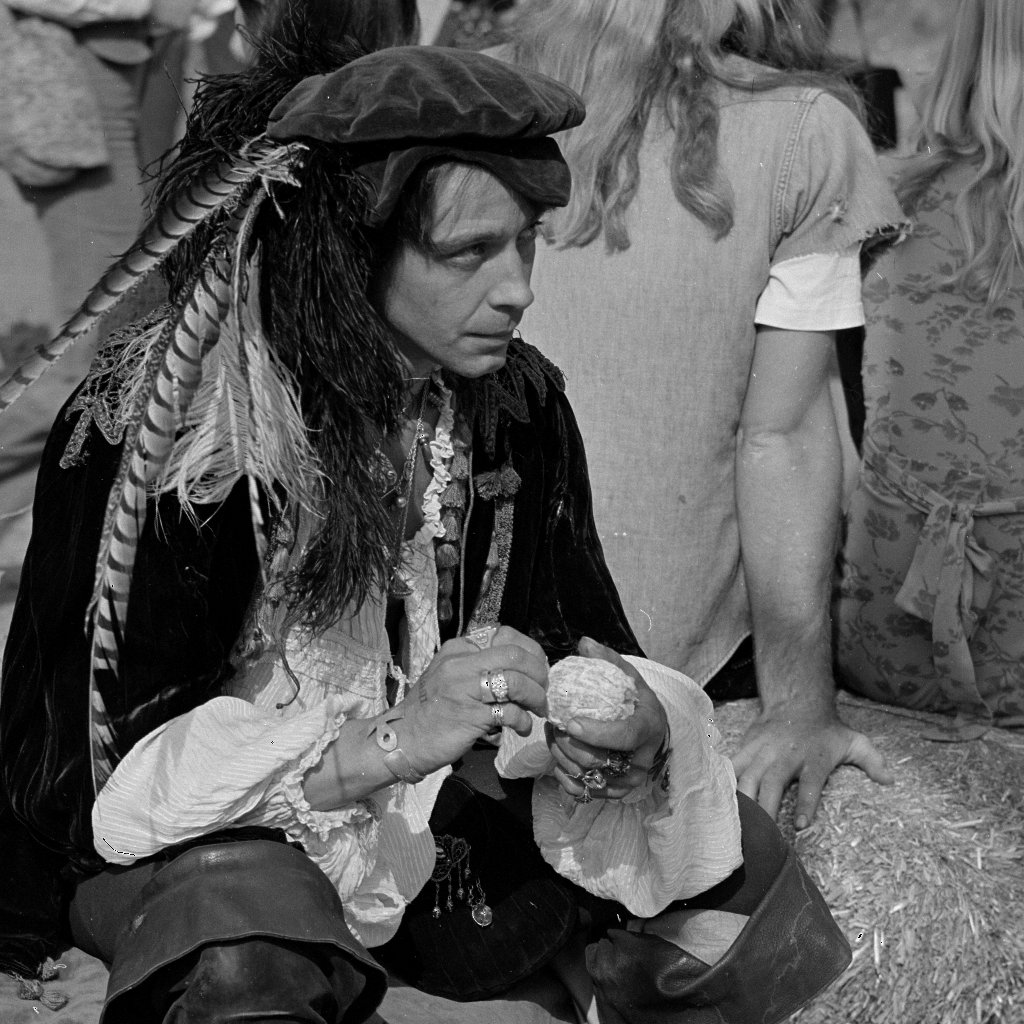
\includegraphics[width=\textwidth]{images/improved_stego_variable_grayingray.png}
        \caption{Stego object produced by the embedding of secret.bmp into vessel.bmp using the variable complexity modification.}
        \label{fig:variable_grayingray}
    \end{subfigure}
    \begin{subfigure}[b]{0.3\textwidth}
        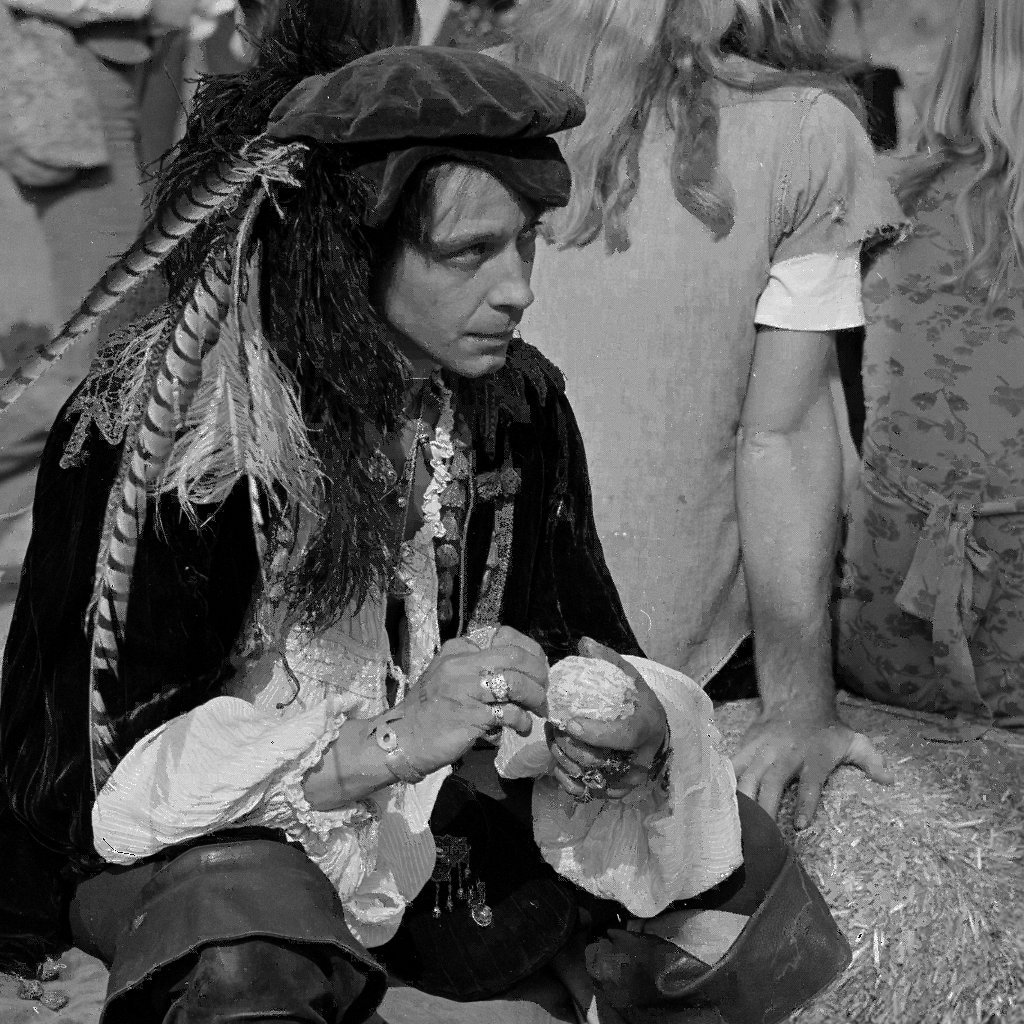
\includegraphics[width=\textwidth]{images/improved_stego_rbeo_grayingray.png}
        \caption{Stego object produced by the embedding of secret.bmp into vessel.bmp using the random bitplane embedding order modification.}
        \label{fig:rbeo_grayingray}
    \end{subfigure}
    \begin{subfigure}[b]{0.3\textwidth}
        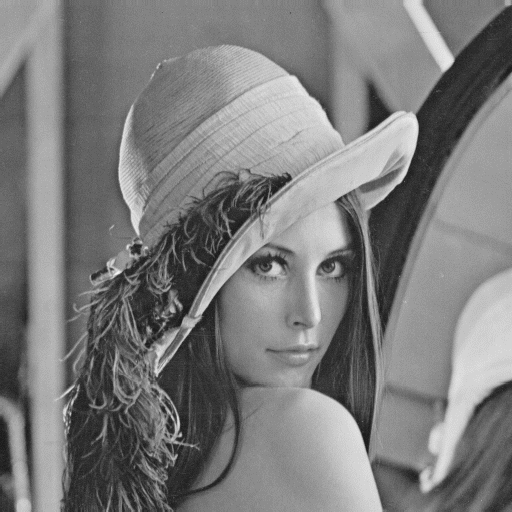
\includegraphics[width=\textwidth]{images/lena.png}
        \caption{Payload recovered by BPCS tool decoder using either of the modifications.}
        \label{fig:extracted_modified_grayingray}
    \end{subfigure}
    \caption{Modified algorithm evaluation using an 8-bit colour payload and 8-bit colour cover. Figure \subref{fig:variable_grayingray} shows the stego object produced by the BPCS encoder from the embedding of the 8-bit colour payload, secret.bmp, in the 8-bit colour cover, vessel.bmp, using the variable complexity modification. Similarly, the stego object produced using the random bitplane embedding order modification is seen in Figure \subref{fig:rbeo_grayingray}. Figure \subref{fig:extracted_modified_grayingray} shows the payload extracted by the BPCS decoder for both of the modifications.}
\end{figure}

Secondly, in the case of a 24-bit colour cover and 8-bit colour payload, we demonstrate using fruit.jpg and lena.bmp respectively. Providing these as parameters to the BPCS tool results in stego objects for each modification seen in figures \textbf{\ref{fig:variable_grayincolour}} and \textbf{\ref{fig:rbeo_grayincolour}}. Using the decoder functionality of the BPCS tool we recover the payload in figure \textbf{\ref{fig:extracted_modified_grayincolour}}, which is the same regardless of modification used.

\begin{figure}[]
    \centering
    \begin{subfigure}[b]{0.3\textwidth}
        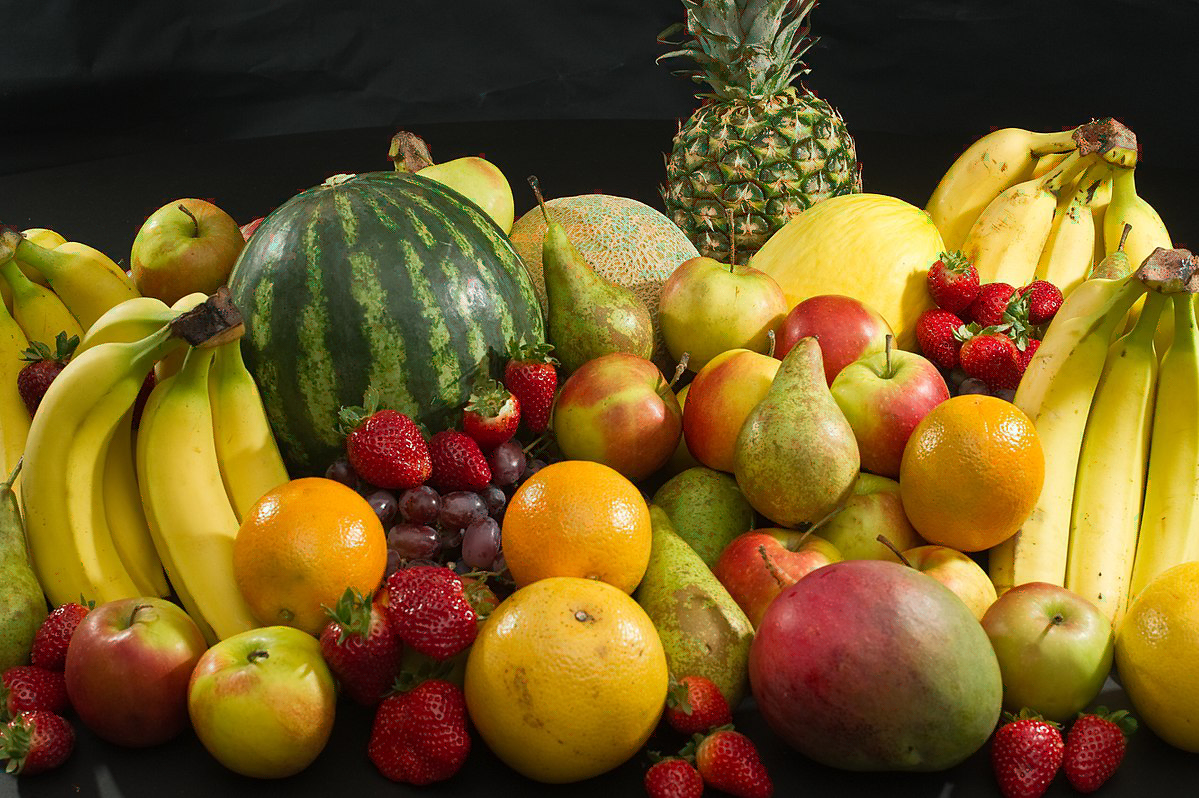
\includegraphics[width=\textwidth]{images/improved_stego_variable_grayincolour.png}
        \caption{Stego object produced by the embedding of lena.bmp into fruit.jpg using the variable complexity modification.}
        \label{fig:variable_grayincolour}
    \end{subfigure}
    \begin{subfigure}[b]{0.3\textwidth}
        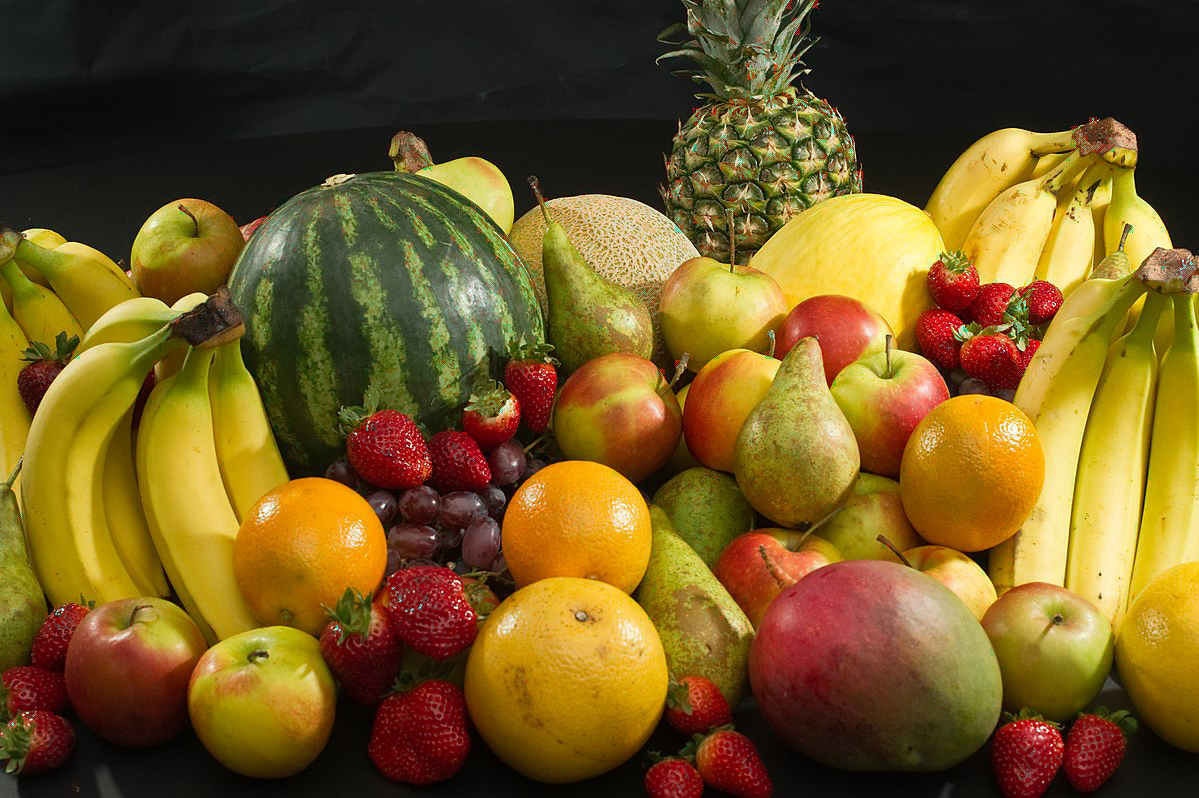
\includegraphics[width=\textwidth]{images/improved_stego_rbeo_grayincolour.png}
        \caption{Stego object produced by the embedding of lena.bmp into fruit.jpg using the random bitplane embedding order modification.}
        \label{fig:rbeo_grayincolour}
    \end{subfigure}
    \begin{subfigure}[b]{0.3\textwidth}
        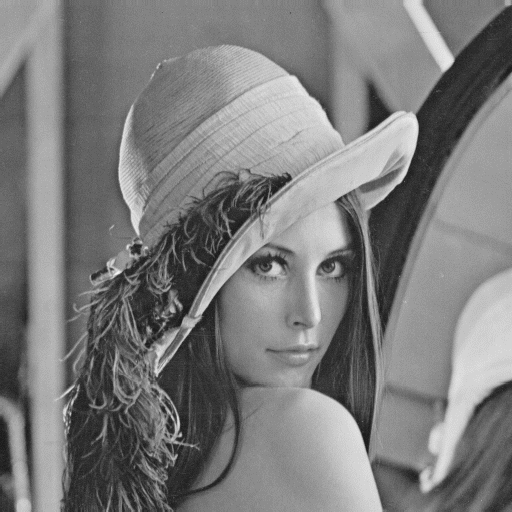
\includegraphics[width=\textwidth]{images/lena.png}
        \caption{Payload recovered by BPCS tool decoder using either of the modifications.}
        \label{fig:extracted_modified_grayincolour}
    \end{subfigure}
    \caption{Modified algorithm evaluation using an 8-bit colour payload and 24-bit colour cover. Figure \subref{fig:variable_grayincolour} shows the stego object produced by the BPCS encoder from the embedding of the 8-bit colour payload, lena.bmp, in the 24-bit colour cover, fruit.jpg, using the variable complexity modification. Similarly, the stego object produced using the random bitplane embedding order modification is seen in Figure \subref{fig:rbeo_grayincolour}. Figure \subref{fig:extracted_modified_grayincolour} shows the payload extracted by the BPCS decoder for both of the modifications.}
\end{figure}

Lastly with two 24-bit colour images, where apple.bmp and green.bmp are the cover and payload respectively. Encoding is performed sequentially for each modification to produce the stego objects seen in figures \textbf{\ref{fig:variable_colourincolour}} and \textbf{\ref{fig:rbeo_colourincolour}}. Following this, the decoder functionality of the BPCS tool recovers the same payload for each modification as seen in figure \textbf{\ref{fig:extracted_modified_colourincolour}}.

\begin{figure}[]
    \centering
    \begin{subfigure}[b]{0.3\textwidth}
        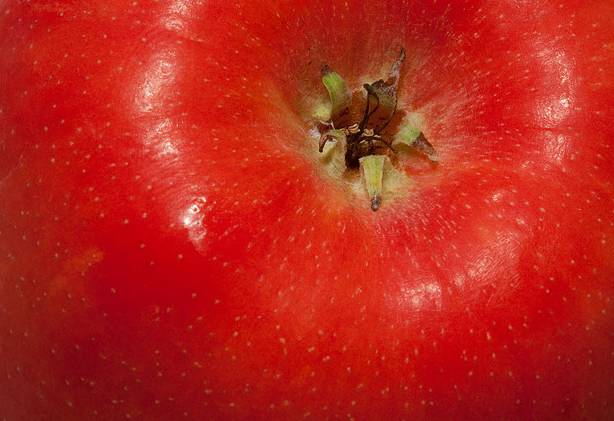
\includegraphics[width=\textwidth]{images/improved_stego_variable_colourincolour.png}
        \caption{Stego object produced by the embedding of green.bmp into apple.bmp using the variable complexity modification.}
        \label{fig:variable_colourincolour}
    \end{subfigure}
    \begin{subfigure}[b]{0.3\textwidth}
        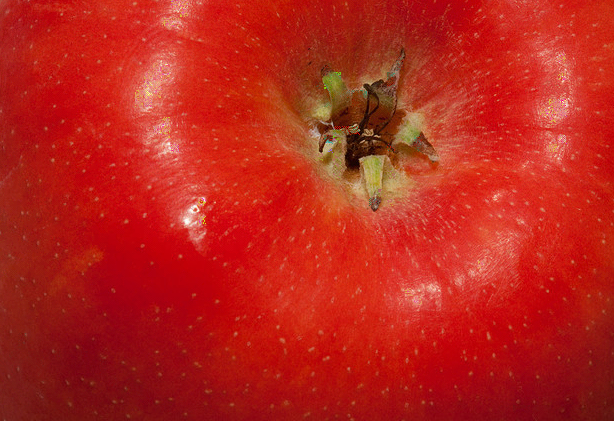
\includegraphics[width=\textwidth]{images/improved_stego_rbeo_colourincolour.png}
        \caption{Stego object produced by the embedding of green.bmp into apple.bmp using the random bitplane embedding order modification.}
        \label{fig:rbeo_colourincolour}
    \end{subfigure}
    \begin{subfigure}[b]{0.3\textwidth}
        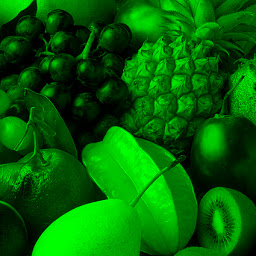
\includegraphics[width=\textwidth]{images/green.png}
        \caption{Payload recovered by BPCS tool decoder using either of the modifications.}
        \label{fig:extracted_modified_colourincolour}
    \end{subfigure}
    \caption{Modified algorithm evaluation using 24-bit colour images. Figure \subref{fig:variable_colourincolour} shows the stego object produced by the BPCS encoder from the embedding of the 24-bit colour payload green.bmp, in the 24-bit colour cover, apple.bmp, using the variable complexity modification. Similarly, the stego object produced using the random bitplane embedding order modification is seen in Figure \subref{fig:rbeo_colourincolour}. Figure \subref{fig:extracted_modified_colourincolour} shows the payload extracted by the BPCS decoder for either of the modifications.}
\end{figure}

The evaluation of the modified algorithm used images of varying colour depths. It was concerned with whether the BPCS tool could successfully perform both embedding and extraction operations of a payload image within a cover object. Through the previous systematic experimentation and a comparison of recovered and original payloads, using the novel developed tool, the evaluation process verified the correctness of the modified algorithm implementation. Hence, meeting the requirement.

\section{Algorithm Comparison}

Previous sections touched only on the correctness of the implementation of BPCS embedding and extraction. However, the pressing matter at hand relates to the likelihood of visual and digital detection. In turn, this opens a discussion into the effects, if any, of the modifications. Briefly, the mechanisms for investigating this are external evaluation and rates of detection using the detection tool. Subsequent sections explain each of these in further detail.

\subsection{Visual Detection}

Importantly the mitigation of bias during evaluation is crucial for an honest assessment of the impact of modifications. Reliance on the modified algorithm developer to evaluate the aspects in question would be unwise, as there is a desired outcome for the results. Other forms of evaluation like a payload comparison tool, digital detection tool and chiefly external participation allow consistent adherence to such a principle.

Appendice section \textbf{\ref{partic}} contains the visual detection evaluation form. Before commencement of any data gathering, participants provided informed consent, following an explanation of the experimentation purpose and method. Appendice section \textbf{\ref{ethics_pdf}} displays the ethical approval for experimentation. Consequently, five individuals took part. Study tasks involved users submitting a verdict on whether they believed that the image currently being viewed contained a hidden payload or not. The study coordinator dictated a randomised viewing order. A randomised order would mitigate any potential learning effects. Learning effects in this context are more consistent identification of embedding signatures as the evaluation progressed. Individuals worked through 24 images categorised into four distinct groups: natural, standard BPCS embedding, variable complexity and random bitplane embedding order. Finally, user's completed a questionnaire of four short questions that aimed to gain an insight into their thought process. 

Figure \textbf{\ref{fig:visual_detection_results}} shows the results of experimentation for each category of an image in terms of the overall percentages of correct and incorrect judgments made by the participants. For natural images, individuals guessed 63.33\% correctly. Participants performed equally well in detecting 43.33\% of hidden payloads for both the standard algorithm and variable complexity modification. RBEO saw the most significant performance by those in the user study, with 96.67\% successful detection by participants. We would expect to see a value of 50\% if participants had guessed rather than follow a consistent strategy. Generally, there were no outliers in terms of individual participant performance, all being of similar standard. 

\begin{figure}
    \centering
    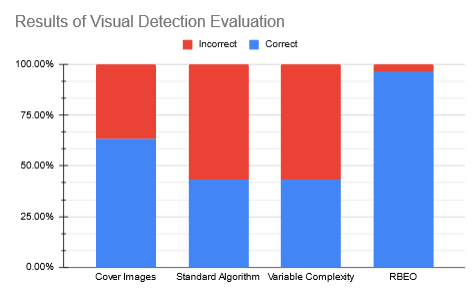
\includegraphics[width=1.0\textwidth]{images/visual_detection_results.png}
    \caption{Results of external visual detection evaluation. Bar graph showing the correct and incorrect judgements for each category of image by all participants.}
    \label{fig:visual_detection_results}
\end{figure}

Explanations for these differences, among categories of images, are apparent from questionnaire responses.  A consensus emerged regarding whether participants deemed themselves capable of identifying the algorithm used to embed a hidden payload. RBEO stood in stark contrast to the other forms of steganography as users felt comfortable spotting the images created using it. Distinguishing between the "standard algorithm" and "variable complexity" modification proved more challenging. Rates of visual detection are highest for RBEO due to the relationship between how it functions and user strategy. Generally, "image artefacts", variance in surrounding pixel colours and "misaligned pixels" informed user judgements. RBEO exacerbates these signatures. Recall the impact of bit-planes on pixel values; LSB has the lowest effect, a change of +1 or -1, and MSB the highest, +128 or -128. Possibly, given the alteration to embedding order with RBEO, more payload data could be present in the MSB than would occur without the modification. Thus, higher impact on pixel values and increased visual degradation. 

As participants worked through the images, an interesting observation arose. Every participant deemed the vessel.bmp to be a stego object despite containing no hidden payload. Deliberation by each individual accompanied repeated phrases of "it doesn't look right", followed by closer inspection of suspect areas. Particular regions of the image: the hair, hands and feathers, were classed as "strange artefacts". However, these observations could not be the result of embedding. Vessel.bmp is a much older image when compared to others in the selection. As a result, we see degradation in the form of creases and discolourations. A perfectly natural example of wearing and tearing was consistently mistaken for signatures of embedding. 

Overall, the results of the visual detection evaluation show positive signs for the variable complexity modification. On the other hand, RBEO is a worsening of performance over the standard algorithm. However, due to the high quantity of user tasks performed during the evaluation, fatigue may have set in. As a result, we address this limitation by performing the next stage of comparison, digital detection.

\subsection{Digital Detection}\label{digital_detection}

As specified in section \textbf{\ref{Analysis}}, an automated tool developed in a language of choice must exist to facilitate the evaluation of the BPCS modifications against the standard algorithm. The key metric from its usage will be the detection rate. The high level design of the detection tool was outlined in section \textbf{\ref{detection_design}} and then implemented as described in section \textbf{\ref{implementation_detection_tool}}. 

When reporting on the detection rate, we isolate the modifications during evaluation to ensure we can attribute causation to any marked improvement seen. Summarising the evaluation procedure as follows. Natural images, stego objects created using the BPCS tool, and the images previously seen in the visual detection phase, serve as parameters to the detection tool.  For each image category, we report measurements, such as the detection rate, true positive, true negative, false positives and false negatives. Compiling these results into tables will draw more attention to findings. One case in the detection tool is of relevance here; stego object only. A separate section, \textbf{\ref{detection_tool_eval}} is reserved specifically for the detection tool and will include the remaining three cases.

We would expect that for each case of a natural image, the detection tool returns a non-stego result. Natural images, alternatively known as "clean" images, are unaltered by something such as our BPCS tool. Hence, they do not contain a payload, and a negative result from the detection tool would reflect this. Table \textbf{\ref{table:detection_results_natural_images}} shows the expected results and actual results for each natural image provided to the detection tool. Likewise, for the stego objects created using the standard algorithm, each is provided to the detection tool. Table \textbf{\ref{table:detection_results_standard_algorithm}} shows the expected results and actual results for each stego object created by the standard algorithm. For the first of our modifications, we look at variable complexity. Table \textbf{\ref{table:detection_results_variable}} shows the expected results and actual results for each stego object created using the variable complexity modification. Regarding the second modification, table \textbf{\ref{table:detection_results_rbeo}} shows the expected results and actual results for each stego object created using the random bitplane embedding order modification.

Aforementioned tables can be collated to produce a summarised group of results seen in table \textbf{\ref{table:detection_results_summarised}}. 
We report absolute values for each set of images on the true positive, true negative, false positive and false negative. Subsequently, detection rates, using these values, are calculated. Identifying the key information from table \textbf{\ref{table:detection_results_summarised}}, we see that for natural images, we achieve a detection rate of 100\%. In the case of standard algorithm stegos, this calculated rate is 100\%. Splitting the modified algorithm into its two distinct components: "variable complexity" and "RBEO", we achieve detection rates of 66\% and 100\%, respectively. 

When devising these modifications, they intended to address the BPCS vulnerability found in external literature, namely the "valley-like" signature appearing in complexity histograms. However, as section \textbf{\ref{implementation_detection_tool}} describes, a shift in steganalysis technique took place, resulting from the failure to reproduce the initial. Herein lies the explanation, for worse than hoped for performance, of the modifications. Crucially, the detection tool operates on a mechanism that had no bearing on the modification design. Variable complexity and RBEO specifically addressed separate components of the valley-like signature. But given the valley is no longer present, modifications have been rendered somewhat redundant. Consider each individually. Recall that the new technique relates to non-zero probabilities of block complexities over 0.9 that only exist from the conjugation operation. Variable complexity will lead to a minor improvement, provided that we set complexity thresholds that do not result in low complexity blocks requiring conjugation. Graphing of a probability distribution of block complexities necessarily includes all bitplanes in the image. RBEO merely changes the order of bitplane embedding, meaning the data we hide, no matter where it is, will still be represented in the plot. As such, with RBEO, we do not address vulnerability exploited in the technique. Thus, RBEO offers no improvement.

Digital detection evaluation isolated each modification. The process was concerned with the impact on the detection rate. Providing the detection tool with natural images, stego objects created using the standard algorithm, stego objects from variable complexity threshold and stego objects from RBEO, results were collected and summarised in tables. A minor improvement arose through the variable complexity modification; 66\% vs 100\% of the standard algorithm, a $\sim$33\% improvement. RBEO did not improve the detection rate, with 100\% of stegos correctly identified by the tool.  We explored what caused this effect. Each modification addressed a vulnerability different to that exploited by the detection tool during evaluation. A more significant improvement could have come by reproducing the "valley-like" signature from existing literature.

\section{JPEG Compression}\label{jpeg_compression}

Given the project's motivation for investigating the impact of lossy compression on steganography, section \textbf{\ref{Analysis}} outlines the need for implementation of the baseline standard of JPEG compression. Section \textbf{\ref{jpeg_design}} provides the high-level design of the JPEG tool, subsequently implemented as described in \textbf{\ref{jpeg_implementation}}. Evaluation of JPEG compression must demonstrate the JPEG tool's capacity to compress both 8-bit and 24-bit colour images.

Summarising the evaluation procedure, we provide the JPEG tool with each image in the test bank as a parameter. In turn, compression steps act on the specified image to produce its respective compressed image. Following this, we can compare the sizes on the disk of the uncompressed and compressed images. A compression ratio is a measure of the relative size of the compressed image compared to the uncompressed. Dividing x by y, where x is the uncompressed size and y is compressed, gives the compression ratio. Table \textbf{\ref{table:jpeg_compression}} presents these values for each image.

\begin{table}[]
\centering
\caption{Evaluation of JPEG compression for images in test bank. Displaying information for original and compressed size as well as calculated compression ratio}
\label{table:jpeg_compression}
\begin{tabular}{@{}lllll@{}}
\toprule
Image    & File Type       & Original Size (kB) & Compressed Size (kB) & Compression Ratio \\\midrule
vessel   & .bmp            & 1000               & 273.5                & 0.2735            \\
secret   & .bmp            & 66.6               & 18.3                 & 0.2748            \\
lena     & .bmp            & 263.2              & 56.2                 & 0.2135            \\
goldhill & .bmp            & 263.2              & 72.1                 & 0.2739            \\
apple    & .bmp            & 776.4              & 82.2                 & 0.1059            \\
fruit    & .jpg            & 223.1              & 343.7                & 1.5406            \\
harry    & .jpg            & 22.5               & 39.1                 & 1.7378            \\
nature   & .jpg            & 25.2               & 38.0                 & 1.5079            \\
green    & .jpg            & 34.5               & 42.4                 & 1.2290            \\\bottomrule
         &                 &                    &                      &                  
\end{tabular}
\end{table}

Depending on the file type of the image supplied to the JPEG tool, we can observe a distinction in compression behaviour. The information in the table reflects a different set of values for .bmp and .jpg images. On average, the compression ratios for .bmp and .jpg images, are 0.228 and 1.504 respectively. What is the reason for such a disparity? The jpeg images sourced online will have already been subject to some form of compression. As we only implemented the baseline JPEG standard, compression steps will be missing in our process. Examples of this would be Huffman encoding and chroma subsampling. The inclusion of these additional steps produces an image of size lower than what can be achieved by the JPEG tool. As such, for .jpg images, we end up with compressed images larger in size relative to their "uncompressed" form - as we lose potential compression from the missing steps that had acted on it previously. 

Compressed image quality can be quantified, in some respect, by the proportion of visual degradation introduced by the algorithm. However, this may be a highly subjective measurement if performed manually by a human. Consequently, we opt for digital analysis using metrics such as mean square error (MSE) and peak signal to noise ratio (PSNR).

Mean Square Error (MSE) represents the average squared difference between pixels in the compressed and uncompressed images. Consider pixel values, from the uncompressed image, of 10 and 20 and pixel values, from the compressed image, of 6 and 8. Firstly, we have a difference of 4 (10-6), yielding a squared difference of 16. Secondly, we have a difference of 12 (20-8) or a squared difference of 144. Hence, an MSE of (12+144)/2, giving 78. Essentially, MSE quantifies how different two images are. Lower MSE values indicate more similarity between the images. The formula for MSE \citep{mseexplanation} is as follows:


\[MSE = \frac{1}{n}\sum_{i=1}^{n}(Y_{i}-Y^{'}_i ) ^2\]

Where: MSE = mean squared error, n = number of data points, \(Y_{i}\) = observed values, \(Y^{'}_i\) = predicted values


Peak signal to noise ratio (PSNR), \citep{psnrform}, is the ratio between the maximum value and data noise. Contextually, we can think of the maximum alternatively known as the peak signal, as the highest pixel value and the noise as our previously calculated mean squared error. Regarding both 8-bit and 24-bit colour images, the maximum value will be 255. 255 is, of course, the maximum number expressable in 8-bit binary representation. Since 24-bit colour images consist of 3 channels, where individually each is 8-bit colour, the maximum values will be the same.

\[PSNR = 20 * log_{10}(\frac{MAX_{i}}{\sqrt{MSE}})\]

Where: PSNR = peak signal to noise ratio, \(MAX_{i}\) = maximum value, MSE = noise in the data (mean squared error) 

Importantly the evaluation procedure must be repeatable and results reproducible. As a result, an automated script calculates the previous metrics for each image in the test bank and produces the graphs seen in figure
\textbf{\ref{compression_metrics_graphs}}. Figure \textbf{\ref{fig:compress_mse_and_psnr}} shows the combined bar graphs of the MSE and PSNR of each image. Figure \textbf{\ref{fig:compress_mse}} shows the MSE only. Figure \textbf{\ref{fig:compress_psnr}} shows the PSNR only. Average metrics values are MSE - 93.75356 and PSNR - 30.38537. 

Externally, typical values for PSNR are 30dB to 50dB \citep{psnrquestion}. Comparing this with the results found previously, PSNR falls within the expected range seen in external literature. As such, the JPEG compression is of sufficient quality. However, there are limitations relating to PSNR's applicability to image evaluation. Noted by \citet{PSNR}, so long as the "content and codec type are not changed [...], PSNR is a reliable measure". While the codec type remains the same, as it is simply the JPEG tool operating on each image, the content is variable. Not all images are the same in their uncompressed state. Due to this, we cannot draw conclusive statements between images since the content is different. As an example, it is invalid to say that vessel.bmp is of higher quality than secret.bmp from its higher PSNR value. Despite this, individual image PSNR values are reflective of those generally regarded as sufficient quality. Thus, PSNR still holds some form of validity in the evaluation.

Evaluation of JPEG compression was concerned with whether the command line application would be capable of compressing an image. A table of results was presented for each image in our test bank, showing the original size, compressed size and a derived compression ratio. A stark contrast exists between the average compression ratios for .bmp and .jpg images. As implementation followed the baseline standard, we miss compression steps that would otherwise have acted on existing online .jpg files. Thus, accounting for the disparity. Judgements regarding the quality of compressed images relate to calculated MSE and PSNR metrics. Despite the limitations listed, the JPEG tool produces images with PSNR values reflective of those seen in external literature. The evaluation process has verified that the JPEG tool can compress both 8-bit and 24-bit colour images.

\section{JPEG Steganography}\label{jpeg_steganography}

As described in section \textbf{\ref{joeg_steganography_implementation}}, JPEG steganography takes place in the spatial domain, in accordance with the requirements laid out in section \textbf{\ref{Analysis}}. In meeting this requirement, the evaluation must demonstrate successful embedding and extraction of a payload within a JPEG compressed image, using any of the implemented techniques. Additionally, we contrast the techniques regarding their effect on visual degradation and embedding capacity.

Summarising the evaluation procedure, we will perform embedding and extraction via the command-line application. Firstly, we compress the cover image followed by the embedding of the desired payload. Secondly,  the JPEG tool decoder performs payload recovery. Each separate instance will be with cover and payload images of varying colour depth. For the three cases, these will be an 8-bit colour cover and payload, a 24-bit colour cover and 8-bit colour payload and lastly, a 24-bit colour cover and payload.  Extracted payload is then compared with the original using the novel comparison tool discussed in previous sections. All steps performed using each of the JPEG steganography algorithms.

In the case of two 8-bit colour images, vessel.bmp and secret.bmp, we embed using each algorithm to produce the respective stego objects seen in figure \textbf{\ref{fig:jpeg_stegos}}. JPEG tool decoder performs payload recovery. Again, we use each algorithm to facilitate this. Figure \textbf{\ref{fig:jpeg_payloads}} provides an overview of each extracted payload.

\begin{figure}
    \centering
    \begin{subfigure}[b]{0.3\textwidth}
        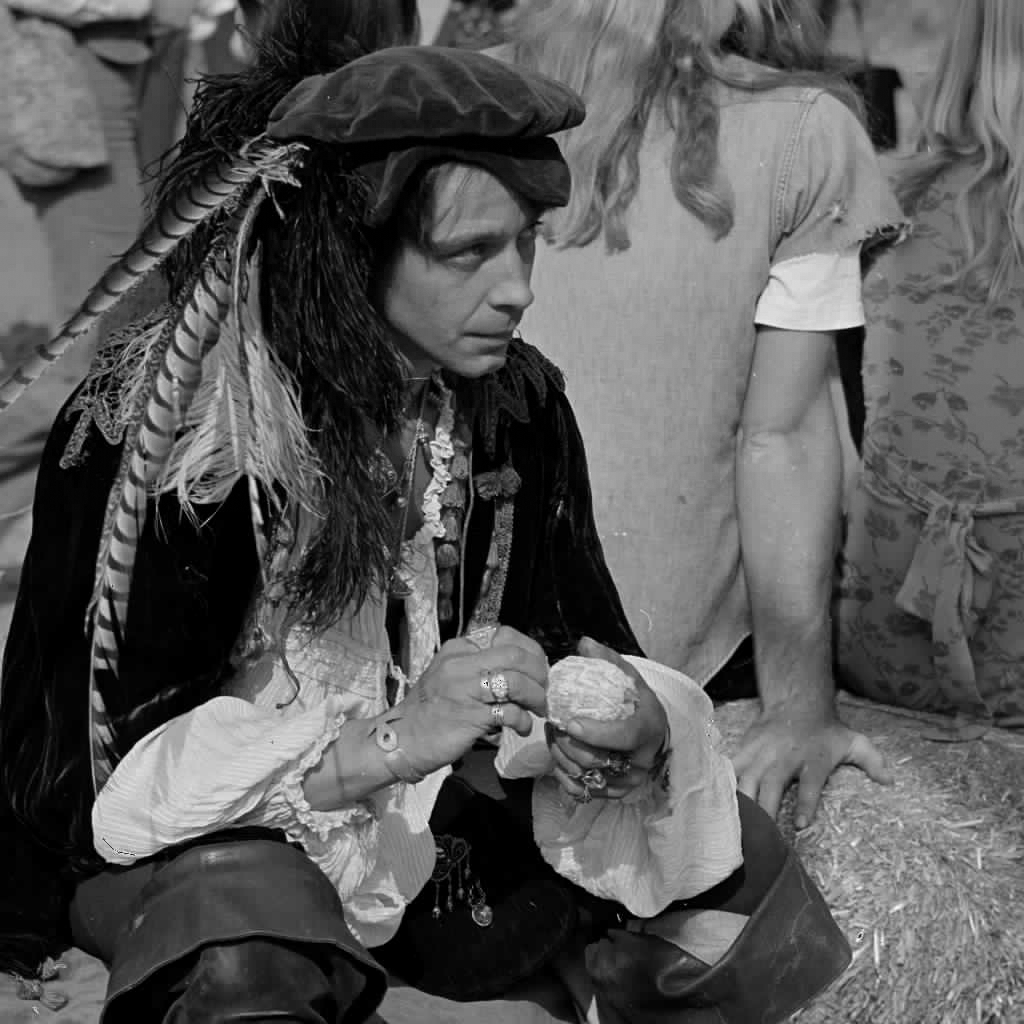
\includegraphics[width=\textwidth]{images/jpeg_steganography_LSB.jpeg}
        \caption{Stego object produced from JPEG LSB steganography}
        \label{fig:jpeg_steg_LSB}
    \end{subfigure}
    \begin{subfigure}[b]{0.3\textwidth}
       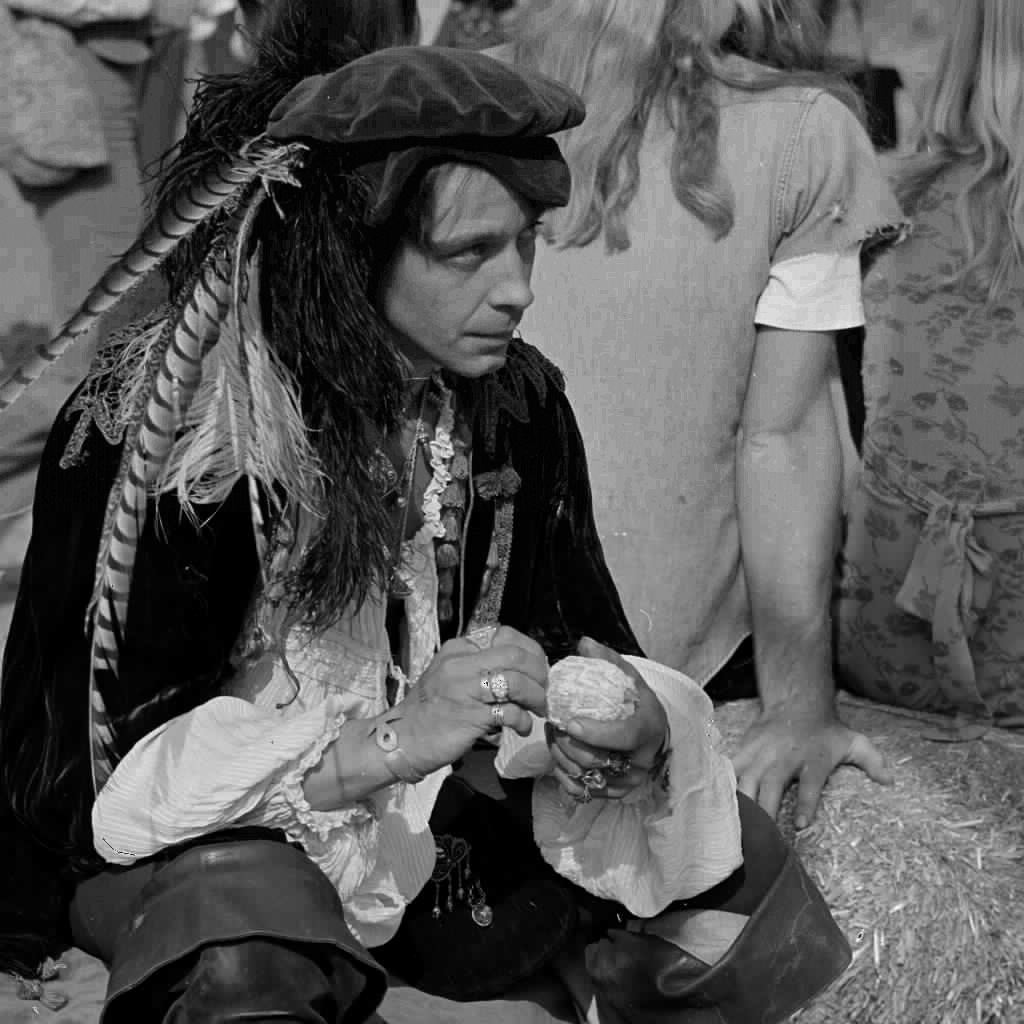
\includegraphics[width=\textwidth]{images/jpeg_steganography_TLSB.jpeg}
        \caption{Stego object produced from JPEG TLSB steganography}
        \label{fig:jpeg_steg_TLSB}
    \end{subfigure}
    \begin{subfigure}[b]{0.3\textwidth}
        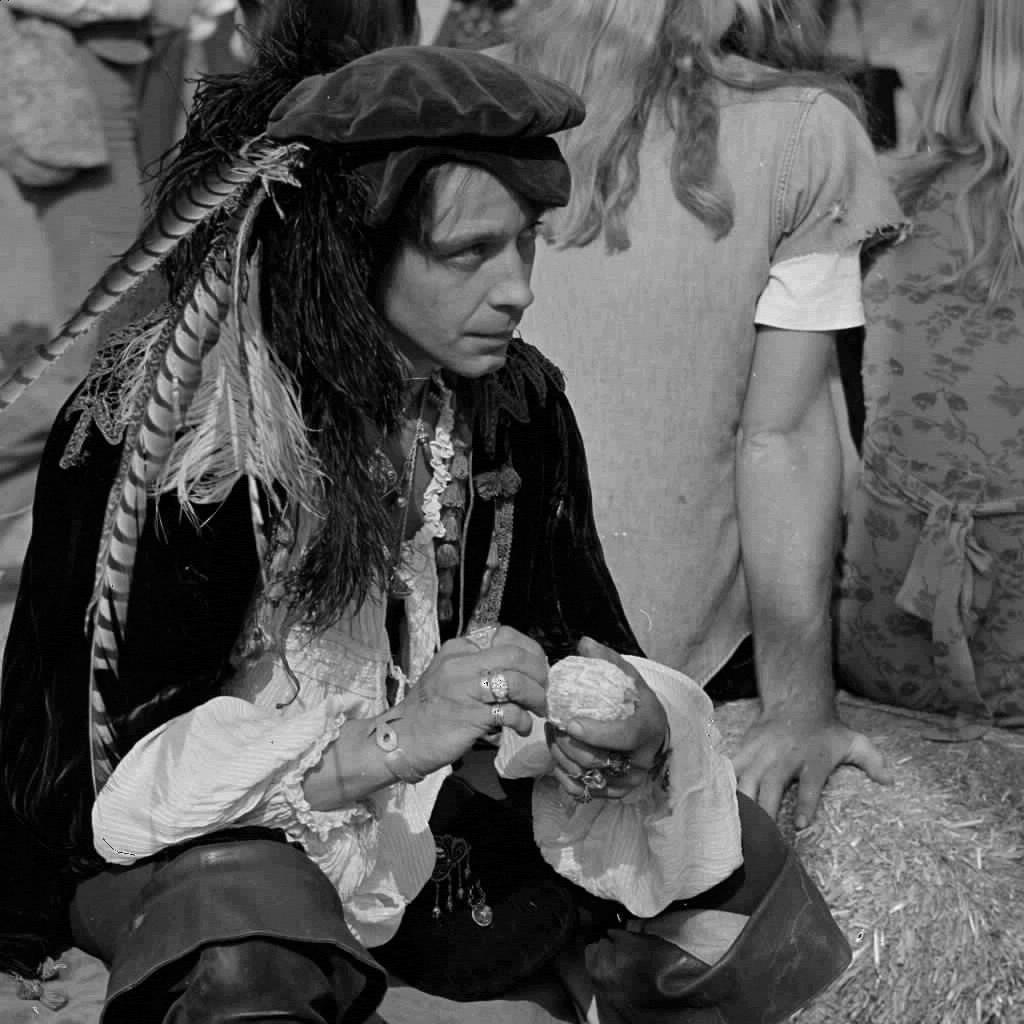
\includegraphics[width=\textwidth]{images/jpeg_steganography_TLSBRandom.jpeg}
        \caption{Stego object produced from JPEG TLSBRandom steganography}
        \label{fig:jpeg_steg_TLSBRandom}
    \end{subfigure}
    \caption{Stego objects produced through JPEG tool embedding of the 8-bit colour payload, secret.bmp, in the 8-bit colour cover, vessel.bmp. Figure \subref{fig:jpeg_steg_LSB} shows the stego image produced using LSB steganography. Figure \subref{fig:jpeg_steg_TLSB} shows the stego image produced using TLSB steganography. Figure \subref{fig:jpeg_steg_TLSBRandom} shows the stego image produced using TLSBRandom steganography.}
    \label{fig:jpeg_stegos}
\end{figure}

Despite the breadth of image types and colour depths covered by the test bank, a problem has arisen. Since each JPEG steganography technique is a variation of LSB embedding, embedding capacity poses a recognisable limitation. LSB enables the replacement of up to 1/8th or 12.5\% of pixels in the cover image. Because of this low embedding capacity, we find that there are only two suitable images usable in evaluation, vessel.bmp and secret.bmp. To test the case of 24-bit colour, we source additional images for the test bank. LSB embedding is not evaluated beyond this point, as it does not function for the previous 8-bit colour images.

In the case of a 24-bit colour cover and 8-bit colour payload, we have our new "wolves.jpeg" and secret.bmp. Embedding is successful, seen by the stego object in figure \textbf{\ref{fig:wolf}}. However, a subsequent attempt at extraction fails. With this in mind, it is redundant to operate for two 24-bit colour images.

Given the operation failure for 24-bit colour images, we focus our technique contrast to 8-bit colour image usage. Comparison of the payloads seen in figure \textbf{\ref{fig:jpeg_payloads}} with the originals results in a clear difference. We have an unsuccessful match for LSB and a successful match for TLSB and TLSBRandom.  Recall the problem of pixel value variance resulting from OpenCV. That is the explanation for the failure of the LSB technique. TLSB and TLSBRandom function as intended.   We would expect TLSBRandom to work, provided that TLSB does so since both are substitutions of the same data only dispersed in a different order.

Evaluation of JPEG steganography was concerned with payload embedding and extraction within a cover object. Of the three implemented techniques, two could achieve this goal. Resulting from the low capacity of LSB embedding, additional images were sourced for the test bank so that evaluation could continue in the case of 24-bit colour images. Ultimately, the usage of a 24-bit colour cover and 8-bit colour payload, and two 24-bit colour images, was unsuccessful. Overall, given the issues arising from low embedding capacity, LSB techniques for JPEG compressed images is less suitable than the previously evaluated BPCS technique.

\begin{figure}
    \centering
    \begin{subfigure}[b]{0.3\textwidth}
        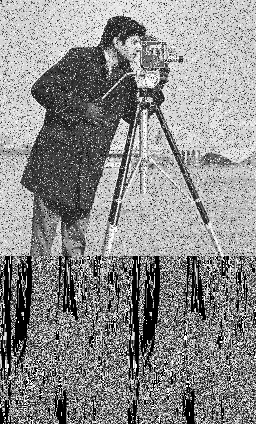
\includegraphics[width=\textwidth]{images/jpeg_steganography_extracted.jpeg}
        \caption{Recovered payload from JPEG LSB steganography}
        \label{fig:jpeg_extracted_LSB}
    \end{subfigure}
    \begin{subfigure}[b]{0.3\textwidth}
        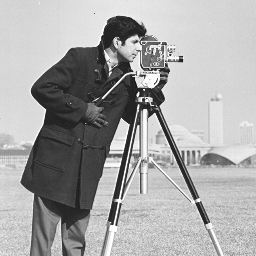
\includegraphics[width=\textwidth]{images/jpeg_steganography_extracted_TLSB.jpeg}
        \caption{Recovered payload from JPEG TLSB steganography}
        \label{fig:jpeg_extracted_TLSB}
    \end{subfigure}
    \begin{subfigure}[b]{0.3\textwidth}
        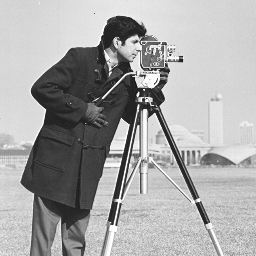
\includegraphics[width=\textwidth]{images/jpeg_steganography_extracted_TLSBRandom.jpeg}
        \caption{Recovered payload from JPEG TLSBRandom steganography}
        \label{fig:jpeg_extracted_LSBRandom}
    \end{subfigure}
    \caption{Payloads recovered using the JPEG tool decoder. Figure \subref{fig:jpeg_steg_LSB} shows the payload recovered using LSB steganography. Figure \subref{fig:jpeg_steg_TLSB} shows the payload recovered using TLSB steganography. Figure \subref{fig:jpeg_steg_TLSBRandom} shows the payload recovered using TLSBRandom steganography }
    \label{fig:jpeg_payloads}
\end{figure}

\section{Detection Tool}\label{detection_tool_eval}

As defined in section \textbf{\ref{Analysis}}, a detection tool must exist capable of detecting the presence of a hidden payload within an image. Demonstration of the requirement necessitates an evaluation of the detection cases involved.  The detection case of a "stego object only" has been covered previously during the digital detection phase of algorithm comparison in section \textbf{\ref{digital_detection}}. Consequently, we focus on the remaining three.

Summarising the evaluation procedure, we create stego objects using the BPCS command-line application. For each detection case, we supply the relevant stego image and additional required parameters. Subsequently, compare the detection tool result with the expected result, e.g. tool indicates no hidden payload despite one being present.

Firstly, in the case of a known cover and stego object. We create three stego objects to reflect the three possible embedding cases. These are secret.bmp in vessel.bmp, secret.bmp in apple.bmp and harry.jpg in fruit.jpg. Detection tool case selected through the command line application with complementary parameters. In each case, we are alerted to the presence of a hidden payload. Following this, we check the possibility of a false-positive result - we do this to ensure the detection tool does not alert the presence, regardless of whether there is a payload or not. Detection tool supplied with a clean cover as both the cover and stego parameters. Leading to a response of no hidden payload detected. Example usage is seen in figure \textbf{\ref{fig:known_cover_and_stego}}, with a false-positive check in figure \textbf{\ref{fig:known_cover_and_stego_falsecheck}}.

Secondly, we have the case of a known payload and stego. Like before, all three colour depth cases are covered using the same images. Again, we select the appropriate detection case in the tool. The actual results are equivalent to our expected results - including a false positive check in the form of secret.bmp embedded in vessel.bmp as stego compared with lena.bmp payload. Example usage is seen in figure \textbf{\ref{fig:known_payload_and_stego}} with a false-positive check in figure \textbf{\ref{fig:known_payload_and_stego_falsecheck}}.

Thirdly we have the case of a known algorithm and stego. Algorithms in this instance are the standard and modified BPCS techniques. Similarly, actual and expected results comparison for each created stego object and algorithm parameter yields the detection tool making the correct judgement. Example usage is seen in figure \textbf{\ref{fig:known_algo_and_stego}} with a false-positive check in figure \textbf{\ref{fig:known_algo_and_stego_falsecheck}}. 

Detection tool evaluation concerned the capability for correctly alerting the presence of a hidden payload in each detection case. Stego objects produced by the BPCS tool, in a variety of colour depths, facilitated comparison of actual results with expected results. At each step, an additional false-positive check ensures the detection tool is not blindly alerting the presence of a hidden payload in every instance. Overall, successful judgements arose every time for each of the detection cases evaluated.

\section{Meeting the Requirements}

The previous sections will have provided evidence demonstrating that requirements relating to each system component have or have not been met. However, there are requirements in the project that are not appropriate for discussion in previous experimentation.

Overall, there are 22 requirements detailed in section \textbf{\ref{Analysis}}, prioritised using the MoSCoW method.  Further splitting this, we have 17 functional requirements, detailed in section \textbf{\ref{functional_requirements}}, and 5 non-functional requirements, detailed in section \textbf{\ref{non_functional_requirements}}. Tables \textbf{\ref{table:meet_requirements_functional}} and \textbf{\ref{table:meet_requirements_non_functional}} lists each requirement, whether it has been met or not and the justification for this. Of these, 14 of 17 functional requirements, $\sim$82\%, and 5 of 5, 100\%, non functional requirements were met. Regarding those not achieved we have: support for 24-bit colour images in JPEG steganography, steps beyond the baseline JPEG standard and a steganographic technique in the frequency domain. In summary, 19 of 22 requirements were met or $\sim$86\%.

\begin{table}[!h]
\centering
\caption{Functional requirements in order of priority and the evidence showing whether they have been met or not.}
\label{table:meet_requirements_functional}
\begin{tabular}{@{}llll@{}}
\toprule
Requirement & Priority & Met? & Evidence                         \\ \midrule
1           & MH       & Y    & Evaluation of Standard Algorithm (Section \textbf{\ref{evaluation_standard_algorithm}}) \\
2           & MH       & Y    & Evaluation of Modified Algorithm (Section  \textbf{\ref{evaluation_modified_algorithm}})\\
3           & MH       & Y    & Evaluation of Detection Tool (Section \textbf{\ref{digital_detection}})\\
4           & MH       & Y    & Evaluation of JPEG Compression (Section \textbf{\ref{jpeg_compression}})\\
5           & MH       & Y    & Evaluation of JPEG Steganography (Section \textbf{\ref{jpeg_steganography}})\\
6           & MH       & Y    & Stego Image: Figure \textbf{\ref{fig:stego_grayingray}}. Recovered Payload: Figure \textbf{\ref{fig:extracted_object}}     \\
7           & MH       & Y    & Use of vessel.bmp in table \textbf{\ref{table:jpeg_compression}}.\\
8           & MH       & Y    & TLSB- Stego Image: Figure \textbf{\ref{fig:jpeg_steg_TLSB}}. Recovered Payload: \textbf{\ref{fig:jpeg_extracted_TLSB}}  \\
9           & MH       & Y    & Section \textbf{\ref{detection_tool_eval}}. 8-bit colour known cover and stego\\ 
10          & SH       & Y    & Evaluation of Modified Algorithm (Section  \textbf{\ref{evaluation_modified_algorithm}})\\
11          & SH       & Y    & Figure \textbf{\ref{fig:compress_mse_and_psnr}}\\
12          & SH       & Y    & Stego Image: Figure \textbf{\ref{fig:stego_colourincolour}}. Recovered Payload: Figure \textbf{\ref{fig:extracted_green}}\\ 
13          & SH       & Y    & Use of apple.bmp in table \textbf{\ref{table:jpeg_compression}}\\ 
14          & SH       & N    &                     \\ 
15          & SH       & Y    & Section \textbf{\ref{detection_tool_eval}}. 24-bit colour known cover and stego\\ 
16          & CH       & N    &                  \\ 
17          & CH       & N    &                 \\\bottomrule     
\end{tabular}
\end{table}

\begin{table}[!h]
\centering
\caption{Non-Functional requirements in order of priority and the evidence showing whether they have been met or not.}
\label{table:meet_requirements_non_functional}
\begin{tabular}{@{}llll@{}}
\toprule
Requirement & Priority & Met? & Evidence                         \\ \midrule
18          & MH       & Y    & Section \textbf{\ref{sphinx}}. Generated docs are in the docs/build directory\\
19          & SH       & Y    & Section \textbf{\ref{command_line}}. High-Level Design in figure \textbf{\ref{Architecture}} \\
20          & SH       & Y    & Section \textbf{\ref{command_line}}. High-Level Design in figure \textbf{\ref{Architecture}} \\
21          & SH       & Y    & Section \textbf{\ref{unit_testing}}. Test Cases are in the src/steganography/tests directory\\
22          & CH       & Y    & Windows 10 and Ubuntu. src/manual.md            \\\bottomrule     
\end{tabular}
\end{table}


%==================================================================================================================================
\chapter{Conclusion}    

This project looked at the BPCS algorithm and steganography in conjunction with lossy compression schemes like JPEG. Project motivation and aims led to subsequent analysis of requirements and conceptualisation of a high-level system design. Such a design served as the bedrock for implementation, followed by an evaluation of system components. Based on the paper, this chapter provides reflective remarks and possible future direction of the project.

\section{Summary}

In summary, steganography is a method of concealing information to perform secret communication. Small capacity techniques like LSB offer simple substitution to accomplish this. Bit-Plane Complexity Segmentation is a different technique that exploits properties of the human visual system. In short, some image regions can hold other data without noticeable changes. Despite the benefits, BPCS possesses vulnerabilities to digital analysis. Through a command-line application, users can perform embedding and extraction operations on secret information using one of two BPCS algorithms; standard and modified. The modified algorithm is composed of two modifications. Firstly, the "variable complexity" modification which varies embedding threshold values, between 0 and 0,45, in each bitplane, rather than a static measure as seen in the standard algorithm. Secondly, the "random bitplane embedding order" modification, RBEO, changes the order of embedding. In the standard algorithm, embedding takes place in the LSB to MSB bitplane. Instead, we use a pseudo-random number generator to create an order.

Determining the effect of these changes required the implementation of a detection tool to facilitate evaluation. This tool operated around four chosen detection cases. The results formed part of a calculated detection rate for the standard algorithm and each modification. Embedding using the standard algorithm resulted in a 100\% detection rate. The inclusion of RBEO did not make any improvement. The variable complexity threshold cut detection down to 66\%. An explanation for poor performance arises from the switch in detection technique. A key signature of BPCS embedding, a "valley-like" signature seen in external literature, could not be reproduced. That led to reliance on an alternative steganalysis technique relating to the block complexity histogram of an image. As well as the digital detection method described previously, evaluation included visual detection involving external participants. Five participants made judgements regarding whether images displayed to them contained hidden payloads. For the variable complexity modification, correct detections were equal to that of the standard algorithm. RBEO performed poorly, with every image detected correctly by a majority of participants. RBEO's poor performance is attributable to its exacerbation of features that participants would look for as part of their detection strategy.

Finally, the project was concerned with steganography in conjunction with lossy compression. Through a command-line application, users can compress an image using the JPEG compression algorithm. Additionally, embedding and extraction operations of a payload can occur. JPEG stenographic techniques revolve around variances in LSB embedding. LSB embedding did not function due to pixel value variances, of at most +1, created by the OpenCV library. TLSB addresses the issue by instead embedding the third least significant bit. It also sets the Second LSB to 0 and LSB to 1 to ensure the variances leave the embedded data unaffected. Overall, LSB is not as suitable as BPCS for performing secret communication. The low embedding capacity meant the test bank required additional images as embedding was impossible in most cases.


\section{Future Work}

Given the poor performance of the modifications in addressing the vulnerabilities, a key area for future work would be to create modifications more suitable for the particular vulnerabilities exploited in the detection tool. An example modification is replacing only half the values in an 8x8 region, with the remaining values left to adjust the complexity measure. Altered complexity measure, if below the chosen threshold in the detection tool, will prevent detection.

Further, attempt to reproduce the BPCS "valley-like" signature in external literature. A repeat digital analysis procedure with the same modifications may result in better performance when using the original technique. The BPCS tool currently informs the user that embedding cannot occur if payload blocks remain after exhausting the complex cover blocks. In the worst-case scenario, a user must wait on the embedding of all blocks, except one. Should alter this to determine if embedding is possible before embedding the blocks, not after.

The system presented in this paper functions as a series of separate command-line applications. The inclusion of a GUI for any of the tools would benefit usability. Rather than typing in image paths manually, a user can instead browse the file directory and select an image. Additionally, the files created by the tools have hard-coded names. As an example, "compressed.jpeg" is the default name of images compressed through the JPEG tool. In future, an additional user argument, after parsing, can set the output file name.

The visual detection phase of algorithm comparison is subject to certain limitations. Untrained participants evaluated the stego images. As a result, individuals did not know, at first, what features to look for as signs of embedding. Learning effects will have had an impact here as participants improve in performance as the evaluation progresses. However, these have been mitigated somewhat through the randomised ordering of images. Usage of trained participants may lead to a further reduction in learning effects. This group would be less likely to guess and consistently follow a strategy compared to untrained participants. Additionally, an increase in the sample group size would benefit results.

Currently, detection tool responsibility is limited to detecting the presence of a payload. It would be beneficial to in future include an option to attempt payload recovery via the tool. With this in mind, a different area of interest would open. Namely, cryptography combined with steganography. If the detection tool could detect and extract a payload, secret communication is compromised. Adding cryptography into one approach ensures that any communication is not compromised. Steganography conceals the information. Cryptography enciphers it.

As revealed by the JPEG steganography evaluation, there is no support for 24-bit colour images.  In future, embedding and extraction, if altered, could allow for the remaining cases. The implemented techniques all concern the spatial domain. One low priority requirement to investigate relates to the inclusion of a frequency domain technique. For JPEG compression, only the baseline JPEG standard, defined in the report, is present in the JPEG tool. Future additions include Huffman encoding and experimentation with chroma subsampling. These additions would lead to further compression, potentially altering the applicable steganography techniques. A "quality factor" parameter, if added, would allow the user to specify the desired quality of the compressed image. Given the problem arising from OpenCV usage, the implementation of a novel encoder would positively impact research. Using byte arrays and manually specifying image headers will eliminate the need for the external library. As a result, the implementation and evaluation of steganography techniques comprise their merit without requiring workarounds.

%==================================================================================================================================
%
% 
%==================================================================================================================================
%  APPENDICES  

\begin{appendices}

\chapter{Ethics Approval}\label{ethics_pdf}

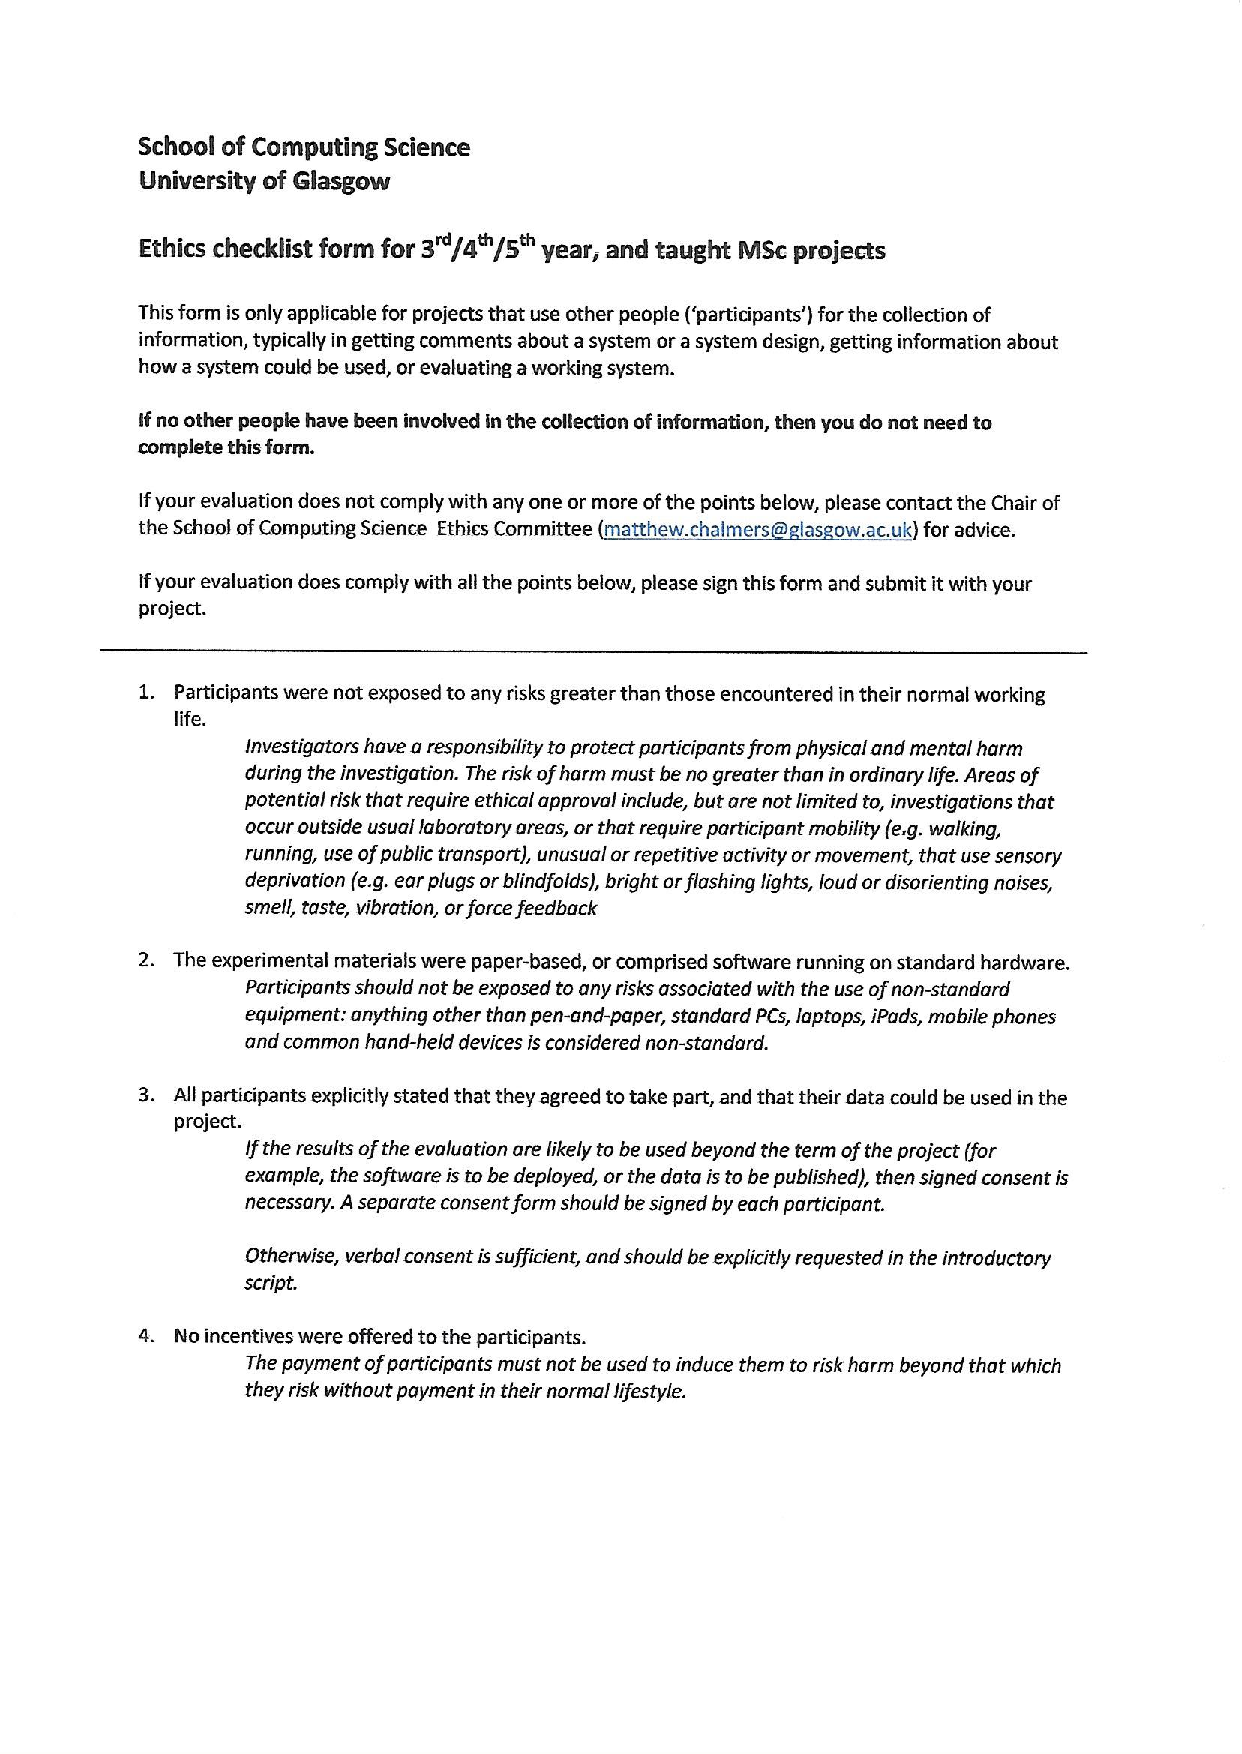
\includepdf[pages=-]{ethics_approval.pdf}

\chapter{Evaluation Form}\label{partic}


\includepdf[pages=-, nup=2x2]{participant_response_form.pdf}

\chapter{Test Images}

\begin{figure}[!h]
    \centering
    \begin{subfigure}[b]{0.3\textwidth}
        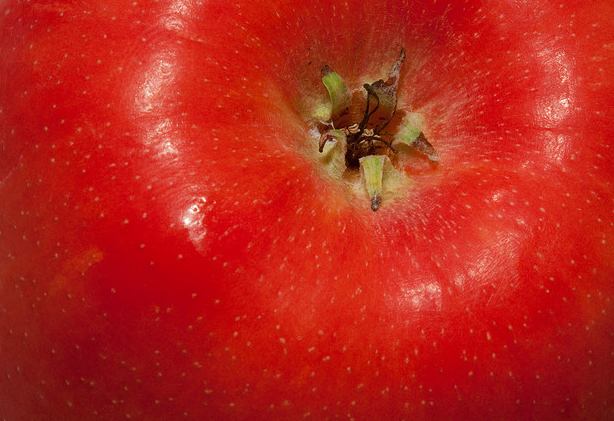
\includegraphics[width=\textwidth]{images/apple.png}
        \caption{apple.bmp}
        \label{apple.bmp}
    \end{subfigure}
    \begin{subfigure}[b]{0.3\textwidth}
        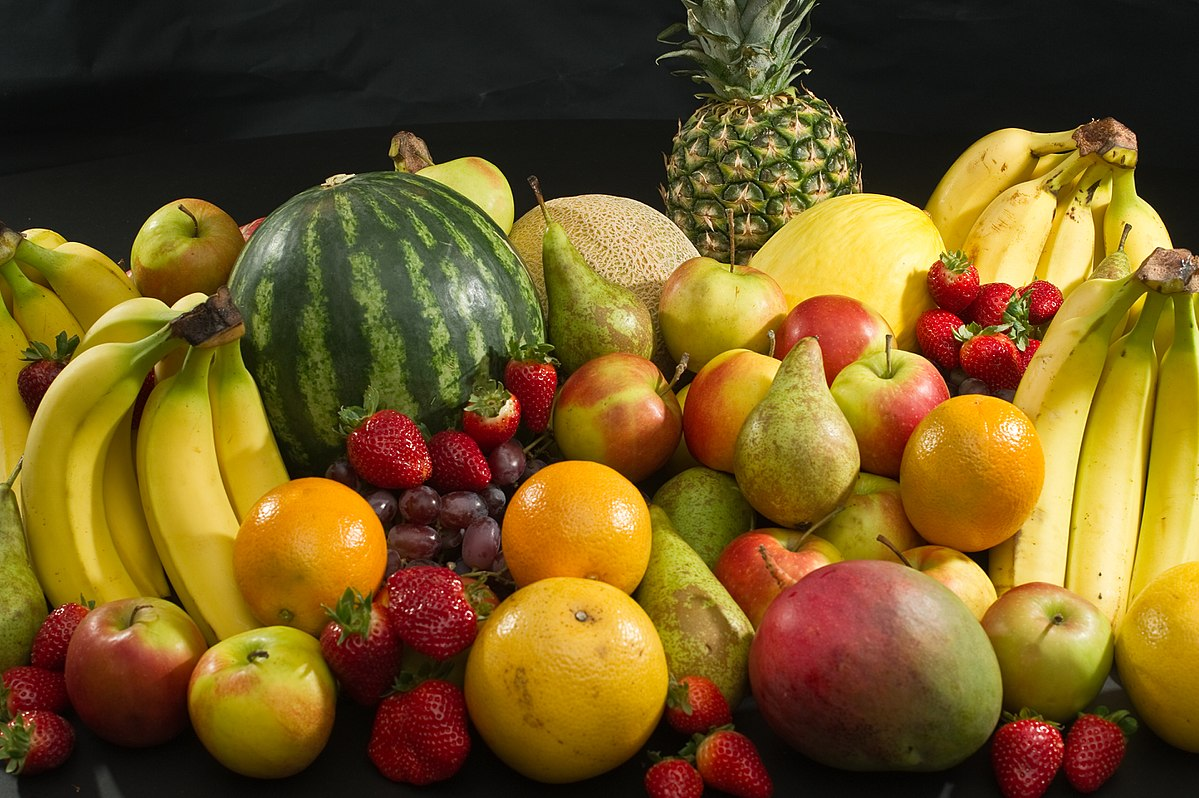
\includegraphics[width=\textwidth]{images/fruit.jpg}
        \caption{fruit.jpg}
        \label{fruit.jpg}
    \end{subfigure}
    \begin{subfigure}[b]{0.3\textwidth}
        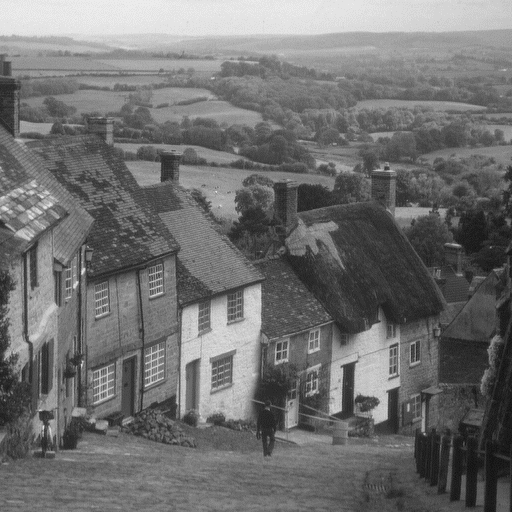
\includegraphics[width=\textwidth]{images/goldhill.png}
        \caption{goldhill.bmp}
        \label{goldhill.bmp}
    \end{subfigure}
    \begin{subfigure}[b]{0.3\textwidth}
        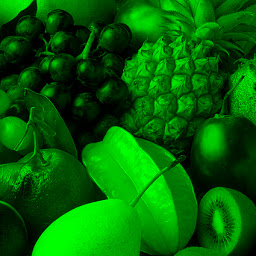
\includegraphics[width=\textwidth]{images/green.png}
        \caption{green.bmp}
        \label{green.bmp}
    \end{subfigure}
    \begin{subfigure}[b]{0.3\textwidth}
        
\includegraphics[width=\textwidth]{images/harry.jpg}
        \caption{harry.jpg}
        \label{harry.jpg}
    \end{subfigure}
    \begin{subfigure}[b]{0.3\textwidth}
        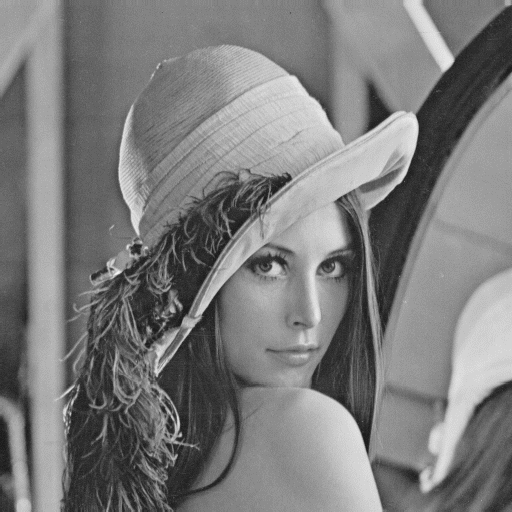
\includegraphics[width=\textwidth]{images/lena.png}
        \caption{lena.bmp}
        \label{lena.png}
    \end{subfigure}
    \begin{subfigure}[b]{0.3\textwidth}
        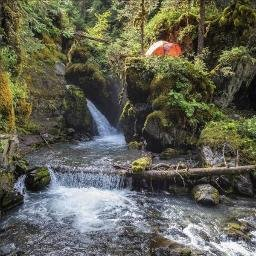
\includegraphics[width=\textwidth]{images/nature.jpg}
        \caption{nature.jpg}
        \label{nature.jpg}
    \end{subfigure}
    \begin{subfigure}[b]{0.3\textwidth}
        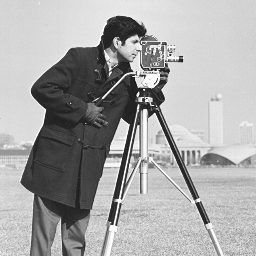
\includegraphics[width=\textwidth]{images/secret.png}
        \caption{secret.bmp}
        \label{secret.bmp}
    \end{subfigure}
    \begin{subfigure}[b]{0.3\textwidth}
        \includegraphics[width=\textwidth]{images/vessel.png}
        \caption{vessel.bmp}
        \label{vessel.bmp}
    \end{subfigure}
    \caption{Test Images}
    \label{fig:test_images}
\end{figure}

\newpage

\chapter{Detection Tool Results}

\begin{table}[!h]
\centering
\caption{Detection Tool Results for Natural Images. Expected values indicate the correct result that we would hope for the detection tool to produce. Actual values are those that the detection tool produces.}
\label{table:detection_results_natural_images}
\begin{tabular}{@{}lll@{}}
\toprule
Natural Image & Expected  & Actual    \\ \midrule
vessel.bmp    & Non-Stego & Non-Stego \\
secret.bmp    & Non-Stego & Non-Stego \\
lena.bmp      & Non-Stego & Non-Stego \\
goldhill.bmp  & Non-Stego &Non-Stego \\
apple.bmp     & Non-Stego & Non-Stego \\
fruit.jpg     & Non-Stego & Non-Stego \\
harry.jpg     & Non-Stego & Non-Stego \\
nature.jpg    & Non-Stego & Non-Stego \\
green.jpg     & Non-Stego & Non-Stego \\ \bottomrule
\end{tabular}
\end{table}

\begin{table}[!h]
\centering
\caption{Detection Tool Results for Standard Algorithm}
\label{table:detection_results_standard_algorithm}
\begin{tabular}{@{}lll@{}}
\toprule
Standard Algorithm      & Expected & Actual    \\ \midrule
vessel.bmp+secret.bmp   & Stego    & Stego     \\
vessel.bmp+lena.bmp     & Stego    & Stego     \\
vessel.bmp+goldhill.bmp & Stego    & Stego     \\
apple.bmp+secret.bmp    & Stego    & Stego     \\
fruit.jpg+green.jpg     & Stego    & Stego \\
fruit.jpg+harry.jpg     & Stego    & Stego     \\ \bottomrule
\end{tabular}
\end{table}

\begin{table}[!h]
\centering
\caption{Detection Tool Results for Variable Complexity Modification}
\label{table:detection_results_variable}
\begin{tabular}{@{}lll@{}}
\toprule
Variable Complexity     & Expected & Actual                \\\midrule
vessel.bmp+secret.bmp   & Stego    & Non-Stego             \\
vessel.bmp+lena.bmp     & Stego    & Stego                 \\
vessel.bmp+goldhill.bmp & Stego    & Stego                 \\
apple.bmp+secret.bmp    & Stego    & Stego                 \\
fruit.jpg+green.jpg     & Stego    & Non-Stego             \\
fruit.jpg+harry.jpg     & Stego    & Stego                \\\bottomrule
\end{tabular}
\end{table}

\begin{table}[!h]
\centering
\caption{Detection Tool Results for Random Bitplane Embedding Order Modification}
\label{table:detection_results_rbeo}
\begin{tabular}{@{}lll@{}}
\toprule
RBEO                    & Expected & Actual \\\midrule
vessel.bmp+secret.bmp   & Stego    & Stego  \\
vessel.bmp+lena.bmp     & Stego    & Stego  \\
vessel.bmp+goldhill.bmp & Stego    & Stego  \\
apple.bmp+secret.bmp    & Stego    & Stego  \\
fruit.jpg+green.jpg     & Stego    & Stego  \\
fruit.jpg+harry.jpg     & Stego    & Stego  \\\bottomrule
\end{tabular}
\end{table}

\begin{table}[!h]
\centering
\caption{Summarised table of results for each set of images.}
\label{table:detection_results_summarised}
\begin{tabular}{@{}llllll@{}}
\toprule
Type                & True Positive & True Negative & False Positive & False Negative & Detection Rate (\%) \\\midrule  \\
Natural Images      &0              &9              &0               &0               &100                   \\
Standard Algorithm  &6              &0              &0               &0               &100                    \\
Variable Complexity &4              &0              &0               &2               &66                    \\
RBEO                &6              &0              &0               &0               &100\\\bottomrule                 
\end{tabular}
\end{table}

\chapter{JPEG Compression Metrics}

\begin{figure}[!h]
    \centering
    \begin{subfigure}[b]{0.55\textwidth}
        \centering
        \includegraphics[width=\linewidth]{images/mse_psnr_combined.png}
        \caption{Combined graph of Mean Square error and peak signal to noise ratio for each image in test bank compressed using JPEG compression}
        \label{fig:compress_mse_and_psnr}
    \end{subfigure}
    \begin{subfigure}[b]{0.55\textwidth}
        \centering
        \includegraphics[width=\linewidth]{images/mse_only.png}
        \caption{Bar Graph of mean square error values for each image in test bank compressed using JPEG Algorithm}
        \label{fig:compress_mse}
    \end{subfigure}
    \begin{subfigure}[b]{0.55\textwidth}
        \centering
        \includegraphics[width=\linewidth]{images/psnr_only.png}
        \caption{Bar Graph of peak signal to noise ratio for each image in test bank compressed using JPEG Algorithm}
        \label{fig:compress_psnr}
    \end{subfigure}
    \caption{Metrics for evaluating JPEG compression. Figure \subref{fig:compress_mse_and_psnr} shows the combined graph of MSE and PSNR. Figure \subref{fig:compress_mse} shows the bar graph of MSE only. Figure \subref{fig:compress_psnr} shows the bar graph of PSNR only.}
    \label{compression_metrics_graphs}
\end{figure}


\chapter{Example Tool Usage}

\section{BPCS Tool Usage}

\subsection{Standard Algorithm}
\begin{figure}[!h]
    \centering
    \begin{subfigure}[b]{0.75\textwidth}
        \includegraphics[width=\textwidth]{images/evaluation_standardbpcs_terminal.png}
        \caption{Example command-line application usage of the BPCS tool encoder during the evaluation of the standard algorithm. The command used runs the encoder with vessel.bmp and secret.bmp images and standard algorithm as parameters.}
        \label{fig:standard_bpcs_encode_terminal}
    \end{subfigure}
    \begin{subfigure}[b]{0.75\textwidth}
        \includegraphics[width=\textwidth]{images/evaluation_standardbpcs_decode_terminal.png}
        \caption{Example command-line application usage of the BPCS tool decoder during the evaluation of the standard algorithm. The command used runs the decoder with stego.bmp and standard algorithm as parameters.}
        \label{fig:standard_bpcs_decoder_terminal}
    \end{subfigure}
    \caption{Example BPCS tool usage during evaluation of standard algorithm. \subref{fig:standard_bpcs_encode_terminal} shows the command line application during the embedding operation. \subref{fig:standard_bpcs_encode_terminal} shows the command line application during the extraction operation.}
\end{figure}

\subsection{Modified Algorithm}\label{modified_use}

\begin{figure}
    \centering
    \begin{subfigure}[b]{0.75\textwidth}
        \includegraphics[width=\textwidth]{images/improved_bpcs_encode_terminal.png}
        \caption{Example command-line application usage of the BPCS tool encoder during the evaluation of the modified algorithm. The command used runs the encoder with vessel.bmp and secret.bmp images and modified algorithm as parameters.}
        \label{fig:improved_bpcs_encode_terminal}
    \end{subfigure}
    \begin{subfigure}[b]{0.75\textwidth}
        \includegraphics[width=\textwidth]{images/improved_bpcs_terminal_decode.png}
        \caption{Example command-line application usage of the BPCS tool decoder during the evaluation of the modified algorithm. The command used runs the decoder with stego.bmp and modified algorithm as parameters}
        \label{fig:improved_bpcs_decoder_terminal}
    \end{subfigure}
    \caption{Example BPCS tool usage during evaluation of the modified algorithm. \subref{fig:improved_bpcs_encode_terminal} shows the command line application during the embedding operation. \subref{fig:improved_bpcs_decoder_terminal} shows the command line application during the extraction operation.}
\end{figure}

\subsubsection{Variable Complexity}

\begin{figure}
    \centering
    \begin{subfigure}[b]{0.75\textwidth}
        \includegraphics[width=\textwidth]{images/vc_terminal_encode.png}
        \caption{Example command-line application usage of the BPCS tool encoder during the evaluation of the variable complexity modification. The command used runs the encoder with vessel.bmp and secret.bmp images and variable complexity modification as parameters.}
        \label{fig:vc_encode_terminal}
    \end{subfigure}
    \begin{subfigure}[b]{0.75\textwidth}
        \includegraphics[width=\textwidth]{images/vc_terminal_decode.png}
        \caption{Example command-line application usage of the BPCS tool decoder during the evaluation of the variable complexity modification. The command used runs the decoder with stego.bmp and variable complexity modification as parameters}
        \label{fig:vc_decode_terminal}
    \end{subfigure}
    \caption{Example BPCS tool usage during evaluation of the variable complexity modification. \subref{fig:vc_encode_terminal} shows the command line application during the embedding operation. \subref{fig:vc_decode_terminal} shows the command line application during the extraction operation.}
\end{figure}

\subsubsection{Random Bitplane Embedding Order}

\begin{figure}
    \centering
    \begin{subfigure}[b]{0.75\textwidth}
        \includegraphics[width=\textwidth]{images/rb_terminal_encode.png}
        \caption{Example command-line application usage of the BPCS tool encoder during the evaluation of the random bitplane embedding order modification. The command used runs the encoder with vessel.bmp and secret.bmp images and random bitplane embedding order modification as parameters.}
        \label{fig:rb_encode_terminal}
    \end{subfigure}
    \begin{subfigure}[b]{0.75\textwidth}
        \includegraphics[width=\textwidth]{images/vc_terminal_decode.png}
        \caption{Example command-line application usage of the BPCS tool decoder during the evaluation of the random bitplane embedding order modification. The command used runs the decoder with stego.bmp and random bitplane embedding orde as parameters}
        \label{fig:rb_decode_terminal}
    \end{subfigure}
    \caption{Example BPCS tool usage during evaluation of the random bitplane embedding order modification. \subref{fig:rb_encode_terminal} shows the command line application during the embedding operation. \subref{fig:rb_decode_terminal} shows the command line application during the extraction operation.}
\end{figure}

\section{Detection Tool Usage}
 \begin{figure}[!h]
    \centering
    \begin{subfigure}[b]{0.75\textwidth}
        \includegraphics[width=\textwidth]{images/evaluation_detection_tool_knowncover.png}
        \caption{Command line application usage for the detection tool in the case of a known cover and stego object.}
        \label{fig:known_cover_and_stego}
    \end{subfigure}
    \begin{subfigure}[b]{0.75\textwidth}
        \includegraphics[width=\textwidth]{images/knowncover_false_check.png}
        \caption{Command line application usage for the detection tool in the case of a false positive check for known cover and stego case.}
        \label{fig:known_cover_and_stego_falsecheck}
    \end{subfigure}
    \caption{Detection tool evaluation in the case of a known cover and stego object. Figure \subref{fig:known_cover_and_stego} shows the command line usage in the case of a known cover and stego for vessel.bmp and secret.bmp embedded in vessel.bmp. Figure \subref{fig:known_cover_and_stego_falsecheck} shows the command line usage in the case of a known cover and stego where vessel.bmp is supplied as both the cover and stego.}
\end{figure}

\begin{figure}[!h]
    \centering
    \begin{subfigure}[b]{0.75\textwidth}
        \includegraphics[width=\textwidth]{images/evaluation_detection_tool_knownpayload.png}
        \caption{Command line application usage for the detection tool in the case of a known payload and stego object.}
        \label{fig:known_payload_and_stego}
    \end{subfigure}
    \begin{subfigure}[b]{0.75\textwidth}
        \includegraphics[width=\textwidth]{images/knownpayload_false_check.png}
        \caption{Command line application usage for the detection tool in the case of a false positive check for a known payload and stego object.}
        \label{fig:known_payload_and_stego_falsecheck}
    \end{subfigure}
    \caption{Detection tool evaluation in the case of a known paylaod and stego object. Figure \subref{fig:known_payload_and_stego} shows the command line usage in the case of a known payload and stego for secret.bmp and secret.bmp embedded in vessel.bmp. Figure \subref{fig:known_payload_and_stego_falsecheck} shows the command line usage in the case of a false payload and stego where lena.bmp is supplied with the stego.bmp containing secret.bmp.}
\end{figure}

\begin{figure}[!h]
    \centering
    \begin{subfigure}[b]{0.75\textwidth}
        \includegraphics[width=\textwidth]{images/evaluation_detection_tool_knownalgo}
        \caption{Command line application usage for the detection tool in the case of a known algorithm and stego object.}
        \label{fig:known_algo_and_stego}
    \end{subfigure}
    \begin{subfigure}[b]{0.75\textwidth}
        \includegraphics[width=\textwidth]{images/knownalgo_false_check.png}
        \caption{Command line application usage for the detection tool in the case of a false positive check for known algorithm and stego object.}
        \label{fig:known_algo_and_stego_falsecheck}
    \end{subfigure}
    \caption{Detection tool evaluation in the case of a known algorithm and stego object. Figure \subref{fig:known_algo_and_stego} shows the command line usage in the case of the known algorithm and stego for secret.bmp embedded in vessel.bmp using the standard algorithm. Figure \subref{fig:known_algo_and_stego_falsecheck} shows the command line usage in the case of a false algorithm and stego  for secret.bmp embedded in vessel.bmp. False algorithm chosen is "modified"}
\end{figure}

\chapter{JPEG Stegos}

\begin{figure}[!h]
    \centering
    \includegraphics[width=0.5\textwidth]{images/wolves.jpg}
    \caption{Stego object produced by LSB embedding of 8-bit colour payload, secret.bmp in 24-bit colour cover wolves.jpeg}
    \label{fig:wolf}
\end{figure}

\end{appendices}

%==================================================================================================================================
%   BIBLIOGRAPHY   

% The bibliography style is abbrvnat
% The bibliography always appears last, after the appendices.

\bibliographystyle{abbrvnat}

\bibliography{l4proj}

\end{document}
